\documentclass[twocolumn,10pt]{ctexart}
% 中文双栏稿件导言区（《自动化学报》/ 中文会议风格）。
% 使用前需有：\documentclass[twocolumn,10pt]{ctexart} 再 % 中文双栏稿件导言区（《自动化学报》/ 中文会议风格）。
% 使用前需有：\documentclass[twocolumn,10pt]{ctexart} 再 % 中文双栏稿件导言区（《自动化学报》/ 中文会议风格）。
% 使用前需有：\documentclass[twocolumn,10pt]{ctexart} 再 \input{preamble}。
\usepackage{amsmath,amssymb,amsthm,mathtools}
\usepackage{graphicx}
\usepackage{booktabs,multirow,array,tabularx}
\usepackage[caption=false]{subfig}
\usepackage{algorithm}
\usepackage{algpseudocode}
\usepackage[margin=2cm]{geometry}
\usepackage{url}
\usepackage{textcomp}
\usepackage{microtype}
\usepackage{bm}
\usepackage[hidelinks]{hyperref}

\setCJKmainfont{Noto Serif CJK SC}[AutoFakeSlant=0.2]
\setCJKsansfont{Noto Sans CJK SC}
\setCJKmonofont{Noto Sans CJK SC}

\graphicspath{{figures/}}
\linespread{1.15}
\setlength{\columnsep}{0.75cm}
\renewcommand{\figurename}{图}
\renewcommand{\tablename}{表}
\renewcommand{\refname}{参考文献}
\renewcommand{\proofname}{证明}
\renewcommand{\abstractname}{摘要}
\floatname{algorithm}{算法}
\algrenewcommand\algorithmicrequire{\textbf{输入：}}
\algrenewcommand\algorithmicensure{\textbf{输出：}}

% 长公式允许跨页断行，避免双栏中的整块溢出。
\allowdisplaybreaks[2]
% 中文行高比西文更高，表格行距略放宽。
\renewcommand{\arraystretch}{1.08}

\newtheorem{theorem}{定理}
\newtheorem{lemma}[theorem]{引理}
\newtheorem{proposition}[theorem]{命题}
\newtheorem{corollary}[theorem]{推论}
\theoremstyle{definition}
\newtheorem{definition}[theorem]{定义}
\newtheorem{assumption}[theorem]{假设}
\newtheorem{example}[theorem]{例}
\theoremstyle{remark}
\newtheorem{remark}[theorem]{注}

\newcommand{\R}{\mathbb{R}}
\newcommand{\Sm}{\mathbb{S}}
\newcommand{\bq}{\mathbf{q}}
\newcommand{\bt}{\mathbf{t}}
\newcommand{\bx}{\mathbf{x}}
\newcommand{\bu}{\mathbf{u}}
\newcommand{\br}{\mathbf{r}}
\newcommand{\bM}{\mathbf{M}}
\newcommand{\bD}{\mathbf{D}}
\newcommand{\bG}{\mathbf{G}}
\newcommand{\bH}{\mathbf{H}}
\newcommand{\bE}{\mathbf{E}}
\newcommand{\bJ}{\mathbf{J}}
\newcommand{\vtwo}{v_2}
\newcommand{\tr}{\operatorname{tr}}
\newcommand{\rank}{\operatorname{rank}}
\newcommand{\diag}{\operatorname{diag}}
\newcommand{\Proj}{\operatorname{Proj}}
\newcommand{\argmin}{\operatorname*{arg\,min}}
。
\usepackage{amsmath,amssymb,amsthm,mathtools}
\usepackage{graphicx}
\usepackage{booktabs,multirow,array,tabularx}
\usepackage[caption=false]{subfig}
\usepackage{algorithm}
\usepackage{algpseudocode}
\usepackage[margin=2cm]{geometry}
\usepackage{url}
\usepackage{textcomp}
\usepackage{microtype}
\usepackage{bm}
\usepackage[hidelinks]{hyperref}

\setCJKmainfont{Noto Serif CJK SC}[AutoFakeSlant=0.2]
\setCJKsansfont{Noto Sans CJK SC}
\setCJKmonofont{Noto Sans CJK SC}

\graphicspath{{figures/}}
\linespread{1.15}
\setlength{\columnsep}{0.75cm}
\renewcommand{\figurename}{图}
\renewcommand{\tablename}{表}
\renewcommand{\refname}{参考文献}
\renewcommand{\proofname}{证明}
\renewcommand{\abstractname}{摘要}
\floatname{algorithm}{算法}
\algrenewcommand\algorithmicrequire{\textbf{输入：}}
\algrenewcommand\algorithmicensure{\textbf{输出：}}

% 长公式允许跨页断行，避免双栏中的整块溢出。
\allowdisplaybreaks[2]
% 中文行高比西文更高，表格行距略放宽。
\renewcommand{\arraystretch}{1.08}

\newtheorem{theorem}{定理}
\newtheorem{lemma}[theorem]{引理}
\newtheorem{proposition}[theorem]{命题}
\newtheorem{corollary}[theorem]{推论}
\theoremstyle{definition}
\newtheorem{definition}[theorem]{定义}
\newtheorem{assumption}[theorem]{假设}
\newtheorem{example}[theorem]{例}
\theoremstyle{remark}
\newtheorem{remark}[theorem]{注}

\newcommand{\R}{\mathbb{R}}
\newcommand{\Sm}{\mathbb{S}}
\newcommand{\bq}{\mathbf{q}}
\newcommand{\bt}{\mathbf{t}}
\newcommand{\bx}{\mathbf{x}}
\newcommand{\bu}{\mathbf{u}}
\newcommand{\br}{\mathbf{r}}
\newcommand{\bM}{\mathbf{M}}
\newcommand{\bD}{\mathbf{D}}
\newcommand{\bG}{\mathbf{G}}
\newcommand{\bH}{\mathbf{H}}
\newcommand{\bE}{\mathbf{E}}
\newcommand{\bJ}{\mathbf{J}}
\newcommand{\vtwo}{v_2}
\newcommand{\tr}{\operatorname{tr}}
\newcommand{\rank}{\operatorname{rank}}
\newcommand{\diag}{\operatorname{diag}}
\newcommand{\Proj}{\operatorname{Proj}}
\newcommand{\argmin}{\operatorname*{arg\,min}}
。
\usepackage{amsmath,amssymb,amsthm,mathtools}
\usepackage{graphicx}
\usepackage{booktabs,multirow,array,tabularx}
\usepackage[caption=false]{subfig}
\usepackage{algorithm}
\usepackage{algpseudocode}
\usepackage[margin=2cm]{geometry}
\usepackage{url}
\usepackage{textcomp}
\usepackage{microtype}
\usepackage{bm}
\usepackage[hidelinks]{hyperref}

\setCJKmainfont{Noto Serif CJK SC}[AutoFakeSlant=0.2]
\setCJKsansfont{Noto Sans CJK SC}
\setCJKmonofont{Noto Sans CJK SC}

\graphicspath{{figures/}}
\linespread{1.15}
\setlength{\columnsep}{0.75cm}
\renewcommand{\figurename}{图}
\renewcommand{\tablename}{表}
\renewcommand{\refname}{参考文献}
\renewcommand{\proofname}{证明}
\renewcommand{\abstractname}{摘要}
\floatname{algorithm}{算法}
\algrenewcommand\algorithmicrequire{\textbf{输入：}}
\algrenewcommand\algorithmicensure{\textbf{输出：}}

% 长公式允许跨页断行，避免双栏中的整块溢出。
\allowdisplaybreaks[2]
% 中文行高比西文更高，表格行距略放宽。
\renewcommand{\arraystretch}{1.08}

\newtheorem{theorem}{定理}
\newtheorem{lemma}[theorem]{引理}
\newtheorem{proposition}[theorem]{命题}
\newtheorem{corollary}[theorem]{推论}
\theoremstyle{definition}
\newtheorem{definition}[theorem]{定义}
\newtheorem{assumption}[theorem]{假设}
\newtheorem{example}[theorem]{例}
\theoremstyle{remark}
\newtheorem{remark}[theorem]{注}

\newcommand{\R}{\mathbb{R}}
\newcommand{\Sm}{\mathbb{S}}
\newcommand{\bq}{\mathbf{q}}
\newcommand{\bt}{\mathbf{t}}
\newcommand{\bx}{\mathbf{x}}
\newcommand{\bu}{\mathbf{u}}
\newcommand{\br}{\mathbf{r}}
\newcommand{\bM}{\mathbf{M}}
\newcommand{\bD}{\mathbf{D}}
\newcommand{\bG}{\mathbf{G}}
\newcommand{\bH}{\mathbf{H}}
\newcommand{\bE}{\mathbf{E}}
\newcommand{\bJ}{\mathbf{J}}
\newcommand{\vtwo}{v_2}
\newcommand{\tr}{\operatorname{tr}}
\newcommand{\rank}{\operatorname{rank}}
\newcommand{\diag}{\operatorname{diag}}
\newcommand{\Proj}{\operatorname{Proj}}
\newcommand{\argmin}{\operatorname*{arg\,min}}


% 浮动体放置：正文共 17 个表格与 5 幅插图，其中多数为双栏浮动体。
% 放宽默认参数，使浮动体尽量排入正文页，而不是被推迟到全文末尾。
\setcounter{topnumber}{4}
\setcounter{bottomnumber}{2}
\setcounter{totalnumber}{6}
\setcounter{dbltopnumber}{3}
\renewcommand{\topfraction}{0.92}
\renewcommand{\bottomfraction}{0.5}
\renewcommand{\textfraction}{0.06}
\renewcommand{\floatpagefraction}{0.6}
\renewcommand{\dbltopfraction}{0.92}
\renewcommand{\dblfloatpagefraction}{0.6}

\begin{document}
\zihao{5}

\title{\zihao{2}\bfseries Laplace-QPEPLayer：基于四元数代数与多模态Laplace平滑的零提升可微位姿估计}
\author{\zihao{4} 第一作者\quad 第二作者\\[2pt] \zihao{5}（[单位名称]，[城市] [邮编]）}
\date{}
\maketitle

\begin{abstract}
\zihao{-5}
可微位姿估计层位于学习式前端与几何后端之间，必须对一个全局最优位姿求导，而该位姿在分支交叉处是不连续的。基于半定规划（SDP）松弛的确定性层在松弛紧时具有可认证性，但需要把问题提升为矩阵变量，并且在两个全局分支交叉时没有定义良好的行为。基于 Boltzmann 分布的概率层避免了硬性分支选择，但通常依赖六维位姿空间中的 Monte Carlo 积分。本文表明，二次位姿估计问题（QPEP）的四元数表述为第三种方案提供了代数结构。对于精确消去平移后剩余的旋转子问题，我们证明：标准 $10$ 维旋转提升恰好等于正交矩阵 $U$ 作用下的 $2Uv_2(q)$；21 条 $SO(3)$ 约束张成的空间恰为 Veronese 簇 $\nu_2(\mathbb{RP}^3)$ 的二次消没理想；相应的 $10\times10$ SDP 是 $\mathbb{S}^3$ 上四次型的 Veronese（Shor）松弛；在一个构造的 Choi--Lam 实例上，认证间隙为 $0.034188$，$\mathrm{rank}(X^\star)=6$。我们推导出闭式 Euler 乘子 $\lambda^\star=4J$，以及 $\mathbb{S}^3$ 上具有精确对映不变性的 $3\times3$ 黎曼隐式微分。将硬 argmin 替换为多模态 Laplace 后验——平移被精确积掉，旋转积分在所有 QPEP 极小点上解析近似，权重为 $w_k\propto e^{-J_k/\tau}/\sqrt{\det H_k}$——得到的层没有 Monte Carlo 方差，推理时无 SDP 提升，反向传播中每个活跃模态只需一次 $3\times3$ 求解。在真实的 LINEMOD 双模态实验中，硬 argmin 的中位旋转误差为 $2.06^\circ$、ADD-S 为 $3.7$ mm，而 Laplace 后验均值被拉向竞争模态（$44.24^\circ$、$13.9$ mm，成对偏差 $+36.9^\circ$）；全次数同伦在 $4/4$ 个实例上确认了通用的 $40$ 个复射影根。

\end{abstract}

\noindent{\zihao{-5}\textbf{关键词：}可微位姿估计；四元数代数；Veronese松弛；Laplace近似；隐式微分；全局优化}

\noindent{\zihao{-5}\textbf{中图分类号：}TP242\quad\textbf{文献标志码：}A}

\section{引言}\label{sec:intro}

几何的端到端学习需要对位姿估计器求导。该估计器是一个具有多个局部极小值的非凸优化问题；一旦全局最小值的身份发生变化，其\emph{全局}解的导数就是一个不连续的对象。目前有两类方法占主导地位，而每一类都在为所得付出代价。

\textbf{确定性全局层。} SDPRLayers \cite{holmes2025sdpr} 将齐次二次约束二次规划（QCQP）提升为矩阵变量 $X\succeq0$，求解 Shor 松弛，并在松弛紧时读出一个秩一的全局解及其对偶证书。其反向传播对原始 QCQP 的 KKT 系统（而不是 SDP）求导，使用一个容忍冗余约束的隐式选择论证。该方法是可认证的，并已在矩阵加权立体定位上得到验证。其代价是结构性的：前向传播在 CPU 上求解 SDP，问题维度随变量数目增长，而保证以紧性和约束规范为条件。对称物体或近平面构型可能产生非紧松弛；此时该层没有位姿可返回。

\textbf{概率层。} EPro-PnP \cite{chen2022epropnp} 将 PnP 残差解释为 $SE(3)$ 上的玻尔兹曼分布，并用 KL 损失、以自适应多重重要性采样训练。这消除了硬分支选择：歧义位姿获得概率质量，梯度在各假设上取平均。其代价是方差：六维蒙特卡罗积分可能漏掉远处的模式，而梯度的方差必须由样本数控制。

\textbf{缺口。} 目前缺少这样一个层：（i）无需凸提升即可全局穷举；（ii）以恒定规模的反向传播可微；（iii）在分支交叉处光滑且无需采样。QPEP 这一工作线 \cite{wu2022qpep} 恰好提供了所需的代数要素：带单一单位范数约束的四元数参数化、平移的精确消去、枚举所有 KKT 根的 Gr\"obner 基求解器，以及闭式的可观测性与协方差分析。QPEP 没有提供的，是对数据的导数以及对歧义的概率处理。

本文在这些要素之上构建 \textsc{Laplace-QPEPLayer}。优化变量为 $q\in\mathbb{S}^3$；平移以闭式消去；前向传播枚举所有实 KKT 根；反向传播使用 $3\times3$ 黎曼隐式微分；歧义由枚举极小值上玻尔兹曼后验的 Laplace 近似处理。该设计刻意保持狭窄：我们不处理不等式约束（伴随线 \textsc{Constrained-QPEPLayer}）或鲁棒外点核（伴随线 \textsc{Robust-QPEPLayer}）。

\subsection{贡献}

\begin{enumerate}
\item \textbf{旋转子问题的精确代数桥梁。} 我们证明齐次旋转提升满足 $x_R(q)=2Uv_2(q)$，其中 $U\in O(10)$（定理~\ref{thm:lift}）；21 个标准 $SO(3)$ 约束恰好张成 $\nu_2(\mathbb{RP}^3)$ 的二次消失理想（定理~\ref{thm:ideal}）；并且相关的 $10\times10$ SDP 是 $\mathbb{S}^3$ 上四次型的 Veronese（Shor）松弛（定理~\ref{thm:sdp}）。适用范围是明确的：这是\emph{精确消去平移之后的旋转子问题}。它覆盖具有完整 20 维理想的 $13\times13$ SDP，我们证明后者等价于 $10\times10$ 的 SDP（定理~\ref{thm:thirteen}），但不覆盖已发布的 $24$ 约束实现——该实现的约束张成空间是 17 维，且一般而言严格更松。
\item \textbf{恒定规模的黎曼反向传播。} 我们由欧拉齐次性、黎曼 Hessian $H_{\mathbb{S}^3}=E^\top(\nabla^2J-4JI)E$ 以及 $q^\star$ 与 $t^\star$ 的隐式 Jacobian 导出 $\lambda^\star=4J$（定理~\ref{thm:implicit}），并具有精确的对映不变性：每个活跃模式一次 $3\times3$ 正定求解，而不是带冗余约束的 KKT 系统。
\item \textbf{多模态、免采样的 Laplace 层。} 平移被精确积掉；旋转通过所有枚举极小值上的 Laplace 近似处理，给出解析权重与梯度（定理~\ref{thm:laplace}）。我们给出正确的测度与归一化常数，证明远离分岔时旋转误差为 $O(\tau)$，并指出近似在何处失效。
\item \textbf{可微性证书，以及诚实的失效分析。} 我们给出 $C^\infty$ 全局位姿映射的充分条件（定理~\ref{thm:cert}），用反例说明一个自然的“精确当且仅当”命题并不成立，并隔离出需要一致渐近的分支合并机制。此外还有：一个带认证间隙的构造 Choi--Lam 实例、一个把已发布松弛与完整理想松弛分离的物理六点反例，以及与理论配套的可复现验证套件。
\end{enumerate}

\subsection{范围，以及我们不主张的内容}\label{sec:nonclaims}

本文的实证部分是对机制、正确性与偏差的受控研究，而不是感知系统的基准。具体来说：

\begin{itemize}
\item 不存在\textbf{检测器级 ADD(-S) 或 ADD-S AUC 主张}，没有基于检测器的旋转或平移误差，没有成功率，也\textbf{没有学习型前端}。第~\ref{sec:real} 节的 LINEMOD 研究直接从真实深度像素与网格顶点构造双模态代价；它是在真实几何上对歧义性、正确性与偏差/光滑性的受控测量。
\item 没有运行任何学习型或可微层基线（SDPR-IS、SDPR-SDP、EPro-PnP、BPnP）。经典 PnP 求解器（EPnP、ITERATIVE、SQPNP、IPPE）与 Theseus 仅作为同一组真实对应关系上的前向与局部参照出现；不附带任何梯度主张。Monte Carlo 基线对离散模式权重采样，并不是 EPro-PnP 的 $SE(3)$ 自适应重要性采样器。
\item UTIAS In-The-Dark 未运行。端到端训练、GPU 批量根枚举、吞吐量与峰值内存均未测量。根枚举的完备性是一个假设（A2），由残差验证而非认证。
\item 认证的 SDP 间隙是数值的（求解器容差下的 PSD 对偶矩阵），而非符号的；并且构造的 Choi--Lam 目标尚不知道能否实现为某个真实对应集的 Gram 矩阵。
\item \textbf{真实数据上的结果是取舍，而不是精度胜利。} 在 15 个真实的近平局帧上，硬 argmin 是准确的（中位数 $2.06^\circ$、$3.7$ mm ADD-S），而 Laplace 后验均值偏向翻转（中位数 $44.24^\circ$、$13.9$ mm、配对偏差 $+36.9^\circ$）。早期出现的 $58.28^\circ$ 这一数字，是把测地线公式作用在\emph{未投影}的 9 维向量平均 $\sum_kw_kR_k$ 上得到的，而后者不是旋转；它不是旋转误差，本文任何地方都不使用它。
\end{itemize}

每个数值主张都标注三种证据级别之一：\emph{论文声明}（在第~\ref{sec:formulation}--\ref{sec:method} 节中给出、且未重新测量）、\emph{独立复现（本仓库）}（由本仓库中的脚本产出，其网格、种子与容差记录在指定的结果文件中；可在此处重跑，而不是对外部论文数字的复现），或\emph{未验证}（没有测量的设计目标）。没有任何论文声明被当作独立复现来呈现。

\section{相关工作}\label{sec:related}

\textbf{可认证层与 SDP 路线。} SDPRLayers \cite{holmes2025sdpr} 将齐次 QCQP 提升为 $X\succeq0$，求解 Shor 松弛，并用一个容忍冗余约束的隐式选择定理对原始 KKT 系统求导。其已发布的位姿估计器使用 $13$ 维向量 $x=[h;\mathrm{vec}(C);t]$ 与 24 个二次约束（6 个正交性、9 个手性、9 个范数），其中最后 18 个被标为冗余。我们的工作在四个方面不同。(i) \emph{变量：}我们在 $q\in\mathbb{S}^3$（四个变量、一个约束）上优化并精确消去 $t$，因此非凸问题的维数是常数，与对应点数目无关。(ii) \emph{全局机制：}QPEP 枚举所有 KKT 根并比较目标值；不存在凸松弛，因而没有紧性假设。(iii) \emph{反向传播：}我们对约化后的平稳性系统用 $3\times3$ 黎曼 Hessian 求导；SDPRLayers 则是在行约化之后对一个带冗余行的 KKT 系统求导。(iv) \emph{歧义：}我们返回模式上的平滑后验；SDPRLayers 返回单个可认证的解，且在松弛不紧时没有定义良好的行为。我们\emph{不}主张我们的 $10\times10$ 分析适用于已发布的 24 约束实现——后者的约束张成空间是 17 维；它确实适用的完整 20D $13\times13$ 松弛，已在定理~\ref{thm:thirteen} 中证明等价于 $10\times10$ 的那一个。

\textbf{概率位姿估计。} EPro-PnP \cite{chen2022epropnp} 在 $SE(3)$ 上定义玻尔兹曼分布，并用自适应多重重要性采样以 KL 损失训练。我们的后验也是玻尔兹曼型，但支撑集是 $\mathbb{S}^3/\{\pm1\}$ 而不是 $SE(3)$，平移被精确边缘化，旋转积分是在穷举的模式列表上解析近似而非采样。这里的取舍是以偏差换方差：EPro-PnP 渐近精确但方差高，而我们的层是确定性的，但在远离分岔处带有 $O(\tau)$ 的 Laplace 偏差。公平的比较必须区分这两个误差来源，而第~\ref{sec:experiments} 节并不声称已做到这一点：只测量了离散模式采样的方差。

\textbf{QPEP 求解器。} Wu \emph{等} \cite{wu2022qpep} 把一大类位姿问题统一为单位四元数中的二次问题，消去平移，用 Gr\"obner 基求解所得多项式系统，并分析可解性、可观测性与协方差。其求解器在已发布实现中至多返回 40 个候选复根（通用的 40 根计数由第~\ref{sec:rootcount} 节的总度同伦确认）；全局解通过比较目标值获得，而不是由凸证书给出。QPEP 没有提供对数据的导数。我们的贡献正是那个缺失的可微层：闭式欧拉乘子、$3\times3$ 隐式微分、对映不变性，以及枚举根上的 Laplace 后验。我们依靠 QPEP 完成前向枚举，并把其完备性作为显式假设（A2）处理。

\textbf{局部求解器的隐式微分。} BPnP \cite{chen2020bpn} 通过对其最优性条件做隐式微分，从而穿过 PnP 求解器反向传播。该求解器是局部的，并由网络预测初始化；所得梯度是局部解的梯度，而不是全局解的梯度。在分支交叉处，局部解可能是错误的那一个，而全局 argmin 的导数作为经典函数并不存在。Theseus \cite{pineda2022theseus} 提供一个可微的非线性最小二乘库，支持李群、稀疏求解器、批处理以及隐式/直接损失最小化；它是一个通用局部优化器，不枚举全局模式，也不提供证书。我们的层更窄（四元数中的四次型代价），但它是穷举的，且反向传播为恒定规模的闭式。

\textbf{多项式优化、矩与平方和。} 我们分析的松弛是二阶 Shor/Veronese 松弛，而不是完整的矩层级。Lasserre 的层级 \cite{lasserre2001} 与 Laurent 的综述 \cite{laurent2009} 给出了一般的矩/SOS 框架；Hilbert \cite{hilbert1888} 确立了非负形式不必是平方和，Blekherman \cite{blekherman2006} 量化了非负形式比 SOS 形式多出多少。Choi--Lam 四次型 \cite{choi1977extremal,choi1980zeros} 是该间隙的标准显式见证，这也是我们用它来构造一个带认证松弛间隙的实例的原因；定理~\ref{thm:lift} 背后的 Veronese 簇的代数几何是标准的 \cite{harris1992}。我们要强调我们\emph{不}做的等同：我们的 SDP 不是教科书上带球面定位矩阵的二阶 Lasserre 矩松弛，我们也不对更高阶层级作任何主张。

\textbf{Laplace 渐近与 $SO(3)$ 的几何。} Laplace 近似及其一致（Airy）对应物是经典的渐近展开结果 \cite{bleistein1986,wong1989}；第~\ref{sec:discussion} 节的分支合并分析正是标准展开不再一致的那个退化情形。旋转积分中的测度常数来自 $SO(3)$ 的 Haar 测度与双覆盖 $\mathbb{S}^3\to SO(3)$ \cite{chirikjian2012}。定理~\ref{thm:implicit}--\ref{thm:cert} 背后的隐函数理论是 Dontchev 与 Rockafellar 的理论 \cite{dontchev2009}，而前向枚举的数值方法（阻尼牛顿、Levenberg--Marquardt、KKT 系统）是标准的 \cite{nocedal2006}。

\textbf{相对于伴随线的范围。} 伴随线 \textsc{Constrained-QPEPLayer} 通过增广拉格朗日与 Fischer--Burmeister 归约加入不等式约束（手性、非穿透、视锥）；\textsc{Robust-QPEPLayer} 加入抗外点的核以及 IRLS 权重的曲率修正。本层两者都不假设：其 $M(\theta)$ 可以是任意加权 Gram 矩阵，其理论也不依赖其他工作线中尚未发表的结果。

\section{问题表述与符号}\label{sec:formulation}

令 $q=[q_0,q_1,q_2,q_3]^\top\in\mathbb{R}^4$ 为单位四元数，$R(q)\in SO(3)$ 为相应的旋转。我们使用齐次提升
\begin{equation}
x_R(q)=\big[\|q\|^2,\ \mathrm{vec}(R(q))^\top\big]^\top\in\mathbb{R}^{10},
\label{eq:lift}
\end{equation}
以及 Veronese 向量
\begin{equation}
\begin{split}
v_2(q)=\big[&q_0^2,\ q_1^2,\ q_2^2,\ q_3^2,\ \sqrt2q_0q_1,\ \sqrt2q_0q_2,\ \sqrt2q_0q_3,\\
&\sqrt2q_1q_2,\ \sqrt2q_1q_3,\ \sqrt2q_2q_3\big]^\top\in\mathbb{R}^{10}.
\end{split}
\label{eq:veronese}
\end{equation}
QPEP 代价族 \cite{wu2022qpep} 为
\begin{equation}
\begin{split}
J_\theta(q,t)={}&v_2(q)^\top M_0(\theta)v_2(q)+2t^\top D(\theta)v_2(q)\\
&+t^\top G(\theta)t,
\end{split}
\label{eq:cost}
\end{equation}
满足 $q^\top q=1$ 且 $G(\theta)\succ0$。消去 $t$ 得到 $t^\star(q)=-G^{-1}Dv_2(q)$ 以及
\begin{equation}
\begin{gathered}
J_{\mathrm{red}}(q;\theta)=v_2(q)^\top M(\theta)v_2(q),\\
M=M_0-D^\top G^{-1}D .
\end{gathered}
\label{eq:reduced}
\end{equation}
映射 $\theta\mapsto(M_0,D,G)$ 假设为 $C^2$（定理~\ref{thm:implicit}）或 $C^3$（定理~\ref{thm:laplace}）。优化变量是四维的；数据只通过固定尺寸的 $10\times10$ 矩阵 $M$ 进入，该矩阵是每次观测组装一次的加权 Gram 矩阵。由于 $v_2$ 是 $\mathrm{Sym}^2(\mathbb{R}^4)$ 的一组基，任何关于 $R(q)$ 各元素为二次的四次型都可以写成 \eqref{eq:reduced} 的形式；这就是该理论所覆盖的函数类。

在驻点 $q^\star$ 处有 $\nabla J=\lambda q$，并且由欧拉齐次性有 $\lambda=4J$（定理~\ref{thm:implicit}）。全文使用的切基为
\begin{equation}
\begin{gathered}
E(q)=\begin{bmatrix}-q_1&-q_2&-q_3\\ q_0&-q_3&q_2\\ q_3&q_0&-q_1\\ -q_2&q_1&q_0\end{bmatrix},\\
q^\top E=0,\qquad E^\top E=I_3,
\end{gathered}
\label{eq:tangent}
\end{equation}
于是切向扰动为 $\delta q=E\,\delta\xi$。对应的旋转向量为 $\omega=2\,\delta\xi$；因此旋转向量坐标下的 Hessian 为 $H_\omega=\tfrac14H_{\mathbb{S}^3}$，即有一个因子 $4$ 把我们的曲率与按单位旋转角表示的曲率分开。QPEP 的可观测性与协方差分析是在其自身参数化下定义的，比较时应按此常数换算。

\textbf{假设。}
\begin{enumerate}
\item[(A1)] 对所考虑的论域中所有 $\theta$，$G(\theta)\succ0$ 且 $M(\theta)\in\mathbb{S}^{10}$。这使 $t^\star$ 唯一，并使约化代价成为球面上定义良好的四次型。
\item[(A2)] 前向代数求解器返回 $\nabla J=4Jq$、$q^\top q=1$ 的\emph{全部}实 KKT 根，直至符号对 $\pm q$。A2 是前向求解器的性质，而不是理论的性质；第~\ref{sec:rootcount} 节测量该系统的通用复根计数，第~\ref{sec:risks} 节说明实验中所用枚举器尚未被验证的部分。
\end{enumerate}

该层或者返回确定性的全局位姿 $(q^{(1)},t^\star(q^{(1)}))$，或者返回枚举极小值 $\{(q^{(k)},w_k)\}_{k=1}^{K}$ 上的平滑后验以及相应的位姿估计。我们记 $\phi=[\mathrm{vec}\,R(q);t^\star(q)]\in\mathbb{R}^{12}$ 为导数经过数值校验的位姿向量，$\Delta J=J(q^{(2)})-J(q^{(1)})$ 为最佳与次佳不同 $SO(3)$ 类之间的目标间隙，$K$ 为 $J_{\mathrm{red}}$ 在 $\mathbb{S}^3/\{\pm1\}$ 上被枚举出的真实局部极小值个数。本文所有旋转误差都是真旋转上的测地角 $\arccos((\operatorname{tr}(R_{\rm est}^\top R_{\rm gt})-1)/2)$，单位为度；所有平移误差都是欧氏误差，单位为米。

\section{方法与理论}\label{sec:method}

\subsection{精确约化与零提升}\label{sec:reduction}

唯一的非线性约束是 $q^\top q=1$。平移被精确消去而非松弛，因此非凸问题化为 $\mathbb{S}^3$ 上的四次型。“零提升”指优化变量：推理时不引入矩阵变量。$10$ 维对象 $v_2$ 与 $x_R$ 是\emph{分析}工具，层内从不在其上优化。

\begin{lemma}[平移的精确消去]\label{lem:translation}
对 $G\succ0$，$\min_t J_\theta(q,t)=J_{\mathrm{red}}(q;\theta)$，在 $t^\star(q)=-G^{-1}Dv_2(q)$ 处取得，并且
\begin{equation}
\begin{split}
\int_{\mathbb{R}^3}e^{-J_\theta(q,t)/\tau}\,dt={}&\frac{(\pi\tau)^{3/2}}{\sqrt{\det G}}\\
&\times e^{-J_{\mathrm{red}}(q;\theta)/\tau}.
\end{split}
\label{eq:gaussint}
\end{equation}
\end{lemma}

\begin{proof}
配方得 $J_\theta(q,t)=(t-t^\star)^\top G(t-t^\star)+J_{\mathrm{red}}(q;\theta)$，其中 $t^\star=-G^{-1}Dv_2(q)$；$\mathbb{R}^3$ 上的高斯积分是标准的。
\end{proof}

\subsection{旋转提升是 Veronese 映射的正交像}\label{sec:lift}

\begin{theorem}\label{thm:lift}
存在 $U\in O(10)$，使得对所有 $q\in\mathbb{R}^4$，
\begin{equation}
\begin{split}
x_R(q)&=2Uv_2(q),\\
\|x_R(q)\|^2&=4\|v_2(q)\|^2=4\|q\|^4 .
\end{split}
\label{eq:bridge}
\end{equation}
\end{theorem}

\begin{proof}[证明梗概]
$x_R$ 的每个元素都是 $q$ 的二次型，而 $v_2$ 是 $\mathrm{Sym}^2(\mathbb{R}^4)$ 的一组基，故存在唯一的 $B$ 使 $x_R=Bv_2$。由于 $R(q)$ 正交，$\|x_R\|^2=\|q\|^4+3\|q\|^4=4\|q\|^4=4\|v_2\|^2$；又 $\{v_2(q)\}$ 张成 $\mathbb{R}^{10}$，故 $B^\top B=4I$。令 $U=B/2$。分块结构是显式的：经行、列置换后，$U=\mathrm{diag}(\tfrac12H_4,\tfrac1{\sqrt2}H_2,\tfrac1{\sqrt2}H_2,\tfrac1{\sqrt2}H_2)$，其中 $H_4$ 为 Sylvester Hadamard 矩阵。
\end{proof}

\textbf{齐次提升。} $x_R$ 必须是\emph{齐次}提升 \eqref{eq:lift}，其首元素为 $\|q\|^2$。若该位置取字面常数 $1$，则恒等式仅在 $\mathbb{S}^3$ 上成立，且 $U$ 在球面外不再正交；齐次提升使定理~\ref{thm:lift} 成为 $\mathbb{R}^4$ 上的恒等式，并使第~\ref{sec:sdp}~节的锥论证成立。

\subsection{21 条 \texorpdfstring{$SO(3)$}{SO(3)} 约束张成二次 Veronese 理想}\label{sec:ideal}

\begin{theorem}\label{thm:ideal}
设 $A_i\in\mathbb{S}^{10}$ 为 21 条标准 $SO(3)$ 约束的矩阵：3 条列范数、3 条列内积、3 条行范数、3 条行内积，以及 9 条齐次叉积方程 $c_a\times c_b-x_0c_c=0$。则
\begin{equation}
\dim\operatorname{span}\{A_i\}=20,
\label{eq:span20}
\end{equation}
并且该张成空间在坐标变换 $x=2Uv_2$ 之后恰为二次消没理想 $\mathcal{I}_2(\nu_2(\mathbb{RP}^3))$。
\end{theorem}

\begin{proof}[证明梗概]
每个 $A_i$ 在 $x_R(\mathbb{S}^3)$ 上为零；其拉回是球面上为零的齐次四次型，因而恒为零，故 $A_i$ 属于映射 $\phi:\mathbb{S}^{10}\to\mathbb{R}[q]_4$，$Q\mapsto Q(x_R(q))$ 的核。$\phi$ 是满射（$R_{ij}$ 的元素张成全部二次型，二次型之积张成全部四次型），故 $\dim\ker\phi=55-35=20$。精确有理秩计算给出 $\operatorname{rank}\{A_i\}=20$；唯一的线性相关是 $\operatorname{tr}(R^\top R)=\operatorname{tr}(RR^\top)$。20 维核中的 20 维子空间即该核。
\end{proof}

\textbf{维数计数与秩计算。} 仅凭维数计数 $55-\binom74=20$ 是必要而不充分的，因为它不能说明 21 个约束矩阵达到该计数；仅凭秩计算也不能把张成空间等同于理想。二者结合才能做到。该计数对约束集敏感：仅六个非对角内积给出秩 15 而非 20，这正是已发布 24 约束实现的约束亏缺并非记账细节的原因。

\subsection{旋转 SDP 是 Veronese 松弛}\label{sec:sdp}

\begin{theorem}\label{thm:sdp}
设 $\{B_k\}_{k=1}^{20}$ 为 $\mathcal{I}_2$ 的一组基，$M\in\mathbb{S}^{10}$。SDP
\begin{equation}
\begin{split}
\min_{Y\succeq0}\ &\langle M,Y\rangle\\
\text{s.t.}\ &\langle B_k,Y\rangle=0\ (k=1,\dots,20),\quad \operatorname{tr}Y=1
\end{split}
\label{eq:sdpY}
\end{equation}
是 $\min_{q\in\mathbb{S}^3}v_2(q)^\top Mv_2(q)$ 的 Shor（Veronese）松弛。在 $x$ 坐标下，令 $Q=\tfrac14UMU^\top$，它等价于
\begin{equation}
\min_{X\succeq0}\ \langle Q,X\rangle\quad\text{s.t.}\quad X_{00}=1,\quad \langle A_i,X\rangle=0,
\label{eq:sdpX}
\end{equation}
其中 $X=4UYU^\top$。
\end{theorem}

\begin{proof}[证明梗概]
两个 PSD 锥由正交合同相联系。在 $(\mathcal{I}_2)^\perp$ 上，$\operatorname{tr}Y=\langle ee^\top,Y\rangle$，$e=(1,1,1,1,0,\dots,0)^\top$，因为两边在秩一生成元 $v_2(q)v_2(q)^\top$ 上一致；又 $U^\top e_0=\tfrac12e$，故 $X_{00}=\langle ee^\top,Y\rangle$。目标值由正交性相等。对偶为 $\max\mu$ s.t. $M-\mu I-\sum_k\lambda_kB_k\succeq0$，即模理想的 SOS 证书。
\end{proof}

\textbf{该等价的范围。} 讨论对象是精确消去平移后的旋转子问题。该 SDP 是二次 Veronese/Shor 松弛，局部化约束是单一的迹/$X_{00}$ 条件，而不是多项式理想的矩矩阵；更高阶松弛不在分析范围内。与已发布 $13\times13$ 实现的关系见定理~\ref{thm:thirteen}。

\subsection{具有认证间隙的构造实例}\label{sec:example}

\begin{example}\label{ex:choilam}
令
\begin{equation}
C(q)=q_0^2q_1^2+q_1^2q_2^2+q_2^2q_0^2+q_3^4-4q_0q_1q_2q_3\ge0,
\label{eq:choilam}
\end{equation}
即 Choi--Lam 非负非 SOS 四次型 \cite{choi1977extremal,choi1980zeros}，并令 $M=M_{CL}+2I_{10}$，其中 $M_{CL}$ 是 $C$ 在 $v_2$ 基下的对称矩阵。真最小值为 $f^\star=2$（因为 $C\ge0$ 且 $\|v_2\|^2=1$）。求解 $10\times10$ 旋转 SDP \eqref{eq:sdpX} 得 $f^\star_{\mathrm{SDP}}=1.9658119658$，对偶证书 $Z=Q-\mu E_{00}-\sum_i\lambda_iA_i$ 满足 $\lambda_{\min}(Z)=-1.8\times10^{-11}$，$\mu=1.9658119658$。因此认证间隙至少为 $0.034188$；原始解满足 $\operatorname{rank}(X^\star)=6$ 与 $\lambda_1/\lambda_2=1.451$。
\end{example}

该实例由本文构造；不同扰动会改变数值间隙与特征值比，因此只报告上述认证实例，表~\ref{tab:sdp_cert} 列出全部量。这里的“认证”指对偶矩阵在求解器容差内为 PSD，而非符号证明。$M$ 能否作为实际 PnP 或矩阵加权对应集的 Gram 矩阵实现，是一个开放问题；第~\ref{sec:thirteen}~节的物理六点实例是互补的可实现分离结果。非负非 SOS 形式的存在性是经典的 \cite{hilbert1888,blekherman2006}，Choi--Lam 形式是标准显式见证；例~\ref{ex:choilam} 的要点不在于这类形式存在，而在于二次 Veronese 松弛会在 QPEP 类中的某个代价上必然失效。

\subsection{\texorpdfstring{$3\times3$}{3x3} 黎曼隐式微分}\label{sec:implicit}

\begin{theorem}\label{thm:implicit}
设 $J(q)=v_2(q)^\top Mv_2(q)$，$q^\star$ 为 $\mathbb{S}^3$ 上的驻点。则：
\begin{enumerate}
\item $\nabla J(q^\star)=\lambda^\star q^\star$，其中 $\lambda^\star=q^{\star\top}\nabla J(q^\star)=4J(q^\star)$。
\item 在基 $E$ 下的黎曼 Hessian 为
\begin{equation}
H_{\mathbb{S}^3}(q^\star)=E(q^\star)^\top\big(\nabla^2J(q^\star)-4J(q^\star)I_4\big)E(q^\star),
\label{eq:hess}
\end{equation}
其中 $\nabla^2J=2J_v^\top MJ_v+2\sum_{a=1}^{10}(Mv_2)_aH_{v,a}$。
\item 若 $H_{\mathbb{S}^3}(q^\star)\succ0$，则局部极小点在 $\theta$ 中局部 $C^\infty$，且
\begin{align}
\frac{\partial q^\star}{\partial\theta}&=-E H_{\mathbb{S}^3}^{-1}E^\top\Big(2J_v^\top\frac{\partial M}{\partial\theta}v_2\Big),\label{eq:dq}\\
\frac{\partial t^\star}{\partial\theta}&=-G^{-1}\Big(\frac{\partial G}{\partial\theta}t^\star+\frac{\partial D}{\partial\theta}v_2+DJ_v\frac{\partial q^\star}{\partial\theta}\Big).\label{eq:dt}
\end{align}
\item 该映射具有对映不变性：$H_{\mathbb{S}^3}(-q^\star)=H_{\mathbb{S}^3}(q^\star)$，$\partial(-q^\star)/\partial\theta=-\partial q^\star/\partial\theta$，且 $\partial\,\mathrm{vec}(R(q^\star))/\partial\theta$ 对 $\pm q^\star$ 相同。
\end{enumerate}
\end{theorem}

\begin{proof}[证明梗概]
Euler 齐次性给出乘子。沿 $\delta q=E\delta\xi$ 对 $F=E^\top\nabla J=0$ 求导，并利用 $(\delta E)^\top q=-E^\top\delta q$，得到 Hessian \eqref{eq:hess}。隐式 Jacobian \eqref{eq:dq}--\eqref{eq:dt} 由对 $F(q^\star(\theta),\theta)=0$ 与 $t^\star=-G^{-1}Dv_2$ 求导得到，即约化驻点系统的隐函数定理 \cite{dontchev2009}。对映不变性来自 $v_2(-q)=v_2(q)$、$J_v(-q)=-J_v(q)$ 与 $E(-q)=-E(q)$。
\end{proof}

\textbf{因子约定。} 这些约定是实现之间产生分歧的常见来源。$\delta q=E\delta\xi$ 对应旋转向量 $2\delta\xi$，故 $H_\omega=\tfrac14H_{\mathbb{S}^3}$，同一协方差在两种约定下的特征值相差因子 16。QPEP 的协方差分析 \cite{wu2022qpep} 使用其自身参数化，比较应在此常数意义下进行。反向传播 \eqref{eq:dq} 对每个活跃模态是一次 $3\times3$ 正定求解，只通过固定的 $4\times10$ Jacobian $J_v$ 接触 $10\times10$ 数据矩阵。

\subsection{可微性证书}\label{sec:cert}

\begin{theorem}[充分条件]\label{thm:cert}
设全局极小在 $q\leftrightarrow-q$ 意义下唯一，$G\succ0$，$H_{\mathbb{S}^3}(q^{(1)})\succ0$，且对次优的不同 $SO(3)$ 类有 $\Delta J=J(q^{(2)})-J(q^{(1)})>0$。则存在 $\theta$ 的邻域，使全局位姿映射在该邻域上 $C^\infty$，其导数由定理~\ref{thm:implicit} 给出。
\end{theorem}

\begin{proof}
隐函数定理给出光滑局部极小；$\Delta J$ 的连续性使其保持全局最优；$G\succ0$ 使 $t^\star$ 唯一。
\end{proof}

\textbf{两个反例界定了该定理。} (i) $\Delta J=0$ 并不排除光滑的全局\emph{选择}：取 $J_1\equiv0$，$J_2(\theta)=(\theta-\theta_0)^2$，则分支 1 对所有 $\theta$ 都是光滑全局极小，尽管两分支在 $\theta_0$ 处打平。正确的命题关乎全局极小的唯一性，而非每个选择的可微性。(ii) $H_{\mathbb{S}^3}\succ0$ 不是必要条件：对 $J(x;\theta)=x^4+\theta^2x^2$，唯一极小 $x^\star(\theta)\equiv0$ 在 $\theta=0$ 处光滑，尽管 Hessian 消失。尖锐的必要条件是约化驻点系统存在一个在每个点都全局最优的可微单值选择；$H\succ0$ 是标准充分条件 \cite{dontchev2009}。

\textbf{QPEP 特有的计数问题。} 朴素计数给出 $K\le27$ 个实极小，该数字没有文献来源，且对于有限根集与自由对映对称 $(q,\lambda)\mapsto(-q,\lambda)$ 不相容。已发布的 LibQPEP 求解器最多返回 40 个候选复根，全次数同伦在 $4/4$ 个实例上确认了 40 个复射影根（带 $\pm$ 双覆盖的 80 个仿射根，第~\ref{sec:rootcount}~节），实射影根数随实例而变。因此我们写“$K$ 个枚举实极小，已发布求解器至多 40 个候选”，把枚举完备性作为假设 (A2)，并以数值方式检验残差。

\subsection{多模态 Laplace 平滑}\label{sec:laplace}

\begin{theorem}\label{thm:laplace}
设 $q^{(k)}$（$k=1,\dots,K$）为 $J_{\mathrm{red}}$ 在 $\mathbb{S}^3/\{\pm1\}$ 上枚举到的非退化局部极小，$H_k=H_{\mathbb{S}^3}(q^{(k)})\succ0$。对 Boltzmann 后验 $p_\theta(q,t)\propto e^{-J_\theta(q,t)/\tau}$：
\begin{enumerate}
\item \textbf{平移是精确的。} $\int_{\mathbb{R}^3}e^{-J_\theta(q,t)/\tau}dt=(\pi\tau)^{3/2}(\det G)^{-1/2}e^{-J_{\mathrm{red}}(q;\theta)/\tau}$。
\item \textbf{旋转用 Laplace 近似。} 以 Haar 测度 $\int_{SO(3)}dR=8\pi^2$ \cite{chirikjian2012}，
\begin{equation}
\begin{split}
&\int_{SO(3)}e^{-J_{\mathrm{red}}/\tau}dR\\
&\quad=8(2\pi\tau)^{3/2}\sum_{k=1}^K\frac{e^{-J_k/\tau}}{\sqrt{\det H_k}}\big(1+O(\tau)\big),
\end{split}
\label{eq:rotationint}
\end{equation}
模态权重为
\begin{equation}
w_k=\operatorname{softmax}_k\Big(-\frac{J_k}{\tau}-\frac12\log\det H_k\Big).
\label{eq:weights}
\end{equation}
\item \textbf{梯度。} 对下游损失 $\ell$，
\begin{equation}
\begin{split}
\nabla_\theta\bar\ell={}&\sum_kw_k\nabla_\theta\ell_k\\
&+\operatorname{Cov}_w\Big(\ell_k,\ -\frac1\tau\nabla_\theta J_k\\
&\qquad-\frac12\nabla_\theta\log\det H_k\Big),
\end{split}
\label{eq:smgrad}
\end{equation}
其中 $\nabla_\theta J_k=v_k^\top(\partial_\theta M)v_k$，且
\begin{equation}
\begin{split}
\nabla_\theta\log\det H_k&=\operatorname{tr}\Big(H_k^{-1}\frac{dH_k}{d\theta}\Big),\\
\frac{dH_k}{d\theta}&=\frac{\partial H}{\partial\theta}\Big|_{q^{(k)}}+\frac{\partial H}{\partial q}\Big|_{q^{(k)}}\frac{\partial q^{(k)}}{\partial\theta}.
\end{split}
\label{eq:dlogdet}
\end{equation}
第二项包含 $J$ 的三阶 $q$ 导数。
\item \textbf{温度极限。} 当 $\tau\to0$ 且 $\Delta J>0$ 时，后验均值与软 argmin 收敛到确定性全局极小，其梯度收敛到定理~\ref{thm:implicit}。KL 损失本身 $\mathcal{L}_{\mathrm{KL}}=\tau^{-1}J_{\mathrm{gt}}+\log Z_{\mathrm{Laplace}}$ 的梯度按 $1/\tau$ 缩放，若不做 $\tau$ 重标定则不发散。
\end{enumerate}
\end{theorem}

\begin{proof}[证明梗概]
平移积分即引理~\ref{lem:translation}。对旋转，在每个 $q^{(k)}$ 附近的正规坐标 $q(u)=\mathrm{normalize}(q^{(k)}+E_ku)$ 中把 $J$ 展开到二阶；高斯积分给出 $(2\pi\tau)^{3/2}(\det H_k)^{-1/2}$。每个叶片的局部 Jacobian 为 $dR=8\,dq$；$\pm q$ 的两个叶片与双覆盖因子 $1/2$ 合起来给出每个 $SO(3)$ 模态的因子 $8$。标准 Laplace 展开给出相对误差 $O(\tau)$ \cite{bleistein1986,wong1989}。梯度公式是对 $J_k$ 用包络定理、对 $w_k$ 用 softmax Jacobian 的链式法则。
\end{proof}

\textbf{分支交叉处的光滑性。} \emph{精确} Boltzmann 后验对每个 $\tau>0$ 都是 $\theta$ 的 $C^\infty$ 函数，因为 $\mathbb{S}^3$ 紧且 $J_\theta$ 光滑（由控制收敛定理可得，无需 $\Delta J>0$）。\emph{Laplace 近似}在交叉处并非一致精确：当 $\Delta J\to0$、$H_k$ 的某个特征值趋于零时，两个 Gauss 分布重叠，$1/\sqrt{\det H_k}$ 权重发散，因此需要一致（Airy）展开，或在合并方向上做一维数值积分 \cite{bleistein1986}。故平滑层对每个 $\tau>0$ 都光滑，而 Laplace 实现仅在远离分岔处具有 $O(\tau)$ 精度。

\textbf{归一化。} 常数影响 $Z$ 但在 $w_k$ 中相消。常用归一化 $Z_{\mathrm{Lap}}=(\pi\tau)^3(\det G)^{-1/2}\sum_k e^{-J_k/\tau}/\sqrt{\det H_k}$ 遗漏了旋转积分的 $2^{3/2}$ 型因子；在 $\tau$ 固定时这是与 $\theta$ 无关的常数，不影响梯度。若改用旋转向量坐标 $\omega=2\delta\xi$，则 $\det H_\omega=\det H_{\mathbb{S}^3}/64$，且必须在 \eqref{eq:weights}--\eqref{eq:dlogdet} 中一致地采用同一种约定。

\subsection{与已发布 \texorpdfstring{$13\times13$}{13x13} 松弛的关系}\label{sec:thirteen}

$10\times10$ 旋转 SDP 与已发布 $13\times13$ SDP 的关系不是单一等式或不等式，而有三层：精确等价、不等式层级，以及严格的物理分离。

\begin{theorem}[三段式 $10\times10$/$13\times13$ 关系]\label{thm:thirteen}
令 $x_{13}=[x_R;t]$，$t\in\mathbb{R}^3$ 不受约束，$Q_{13}=\begin{bmatrix}Q_{RR}&Q_{Rt}\\Q_{Rt}^\top&G\end{bmatrix}$ 且 $G\succ0$，$Q_{10}=Q_{RR}-Q_{Rt}G^{-1}Q_{Rt}^\top$。记 $f^\star_{10,\mathrm{full}}$、$f^\star_{13,\mathrm{full}}$ 与 $f^\star_{13,\mathrm{up}}$ 分别为：(a) 完整 20 维理想下 $10\times10$ 的值；(b) 同一完整理想下 $13\times13$ 的值，即上游 24 条约束加三条行正交方程（27 条约束，20 维）；(c) 已发布 24 条约束下 $13\times13$ 的值，其张成空间为 17 维。则：
\begin{enumerate}
\item \textbf{完整 20 维等价（已证明）。} $\mathbb{S}^{13}$ 中 $SE(3)$ 的二次消没理想为 $\mathcal{I}_2(SE(3))=\mathcal{I}_2(SO(3))\oplus\mathbf{0}_{3\times3}$：维数 20，与 $t$ 无耦合。因此分块 Schur 补双射 $X^\star_{13,\mathrm{full}}=LX^\star_{10,\mathrm{full}}L^\top$（$L=[I_{10};\,-G^{-1}Q_{Rt}^\top]$ 满列秩）给出
\begin{equation}
\begin{split}
f^\star_{13,\mathrm{full}}&\equiv f^\star_{10,\mathrm{full}},\\
\operatorname{rank}\big(X^\star_{13,\mathrm{full}}\big)&\equiv\operatorname{rank}\big(X^\star_{10,\mathrm{full}}\big).
\end{split}
\label{eq:schur}
\end{equation}
这是代数恒等式，而非数值巧合。
\item \textbf{上游 17 维实现更松，且在一般情况下严格更松（已证明）。} 已发布的 24 条约束只张成 20 维中的 17 维，故 $\mathcal{V}_{17}\subsetneq\mathcal{I}_2(SO(3))$，上游可行集严格包含完整 20 维可行集。因此对\emph{每个}实例，
\begin{equation}
f^\star_{13,\mathrm{up}}\;\le\;f^\star_{13,\mathrm{full}}=f^\star_{10,\mathrm{full}}\;\le\;f^\star_{\mathrm{QPEP}},
\label{eq:hierarchy}
\end{equation}
最后一个不等式是定理~\ref{thm:sdp} 的松弛界。由于论证与实例无关，每个不紧的完整 20 维实例自动是已发布实现的非紧实例。
\item \textbf{物理六点分离（已证明并独立复现）。} 第 (2) 层在一个真实的矩阵加权 3D--3D 代价上是严格的，该代价具有正权重与唯一真值旋转，即使完整 20 维 SDP 在秩一处恰好紧（表~\ref{tab:6point}）。由连续性，严格不等式在该实例的开邻域内保持，因此分离不是零测的病理情形。
\end{enumerate}
\end{theorem}

\begin{proof}[证明梗概]
(1) $\mathbb{S}^{13}$ 中 $SE(3)$ 的二次消没理想是 $x_R$ 块中 $SO(3)$ 的理想与自由的 $t$ 块的直和，故与 $t$ 无耦合；代价中的耦合是二次的，由 Schur 补完成，而该补正是映射 $L$。代入 $X_{13}=LX_{10}L^\top$ 使约束与目标不变，且 $G\succ0$ 使 $L$ 满列秩。(2) 当张成集缺少三个维度时，子空间包含是严格的；可行性对更大的可行集单调，\eqref{eq:hierarchy} 的最后一个不等式是标准松弛界。(3) 该实例在第~\ref{sec:results_sdp}~节分析；其精确解在完整理想最优点处满足 $r_1^\top r_2=0$，在上游最优点处满足 $r_1^\top r_2>0$，故包含在该处严格，而严格性是开条件。
\end{proof}

\textbf{约束的精确比较。} $10\times10$ SDP 的 21 条 $SO(3)$ 约束张成 20 维（定理~\ref{thm:ideal}）。$13\times13$ SDP 的 24 条上游约束只张成 17 维；把 21 条约束逐条投影到该 17 维张成空间，恰好留下三个非零残差——行正交方程 $r_1\cdot r_2=r_1\cdot r_3=r_2\cdot r_3=0$（残差 1.63--1.73；其余 18 条 $\le6.2\times10^{-16}$）。行范数 $\|r_i\|^2=h^2$ 已由九条范数约束与列正交性蕴含，因此行点积就是全部亏缺。$13\times13$ 约束生成元由已发布 SDPRLayers 实现逐行复刻，并与上游生成元逐元素比对：24 条约束全部一致（24/24），最大 $|\Delta|=0$，且在随机旋转上 $\max_i|x^\top A_i x|=1.4\times10^{-16}$。该复刻是对本文重实现的检验。度量后果见表~\ref{tab:13v10} 与表~\ref{tab:6point}。

\subsection{算法与复杂度}\label{sec:algorithm}

\begin{algorithm}[t]
\caption{\textsc{Laplace-QPEPLayer} 的前向与反向（单个批元素）。}
\label{alg:layer}
\begin{algorithmic}[1]
\State \textbf{前向：}
\State 由 $\theta$ 构造 $M_0,D,G$；\ $M\gets M_0-D^\top G^{-1}D$
\State 枚举 $\nabla J=4Jq$、$q^\top q=1$ 的全部实 KKT 根 $q^{(k)}$
\State 保留满足 $H_k\succ0$ 的局部极小；按 $J_k$ 排序；按 \eqref{eq:weights} 计算 $w_k$
\State \Return $(q^{(1)},t^\star(q^{(1)}))$ 和/或 $\{(q^{(k)},w_k)\}_{k=1}^{K}$
\State \textbf{反向：}
\For{每个活跃模态 $k$}
  \State 按 \eqref{eq:hess} 构造 $H_k$，按 \eqref{eq:dlogdet} 构造 $dH_k/d\theta$
  \State 解 $H_k\,x=E^\top\big(2J_v^\top(\partial_\theta M)v_2\big)$，并令 $\partial q^{(k)}/\partial\theta=-Ex$
\EndFor
\State 组装确定性 Jacobian \eqref{eq:dq}--\eqref{eq:dt} 或平滑梯度 \eqref{eq:smgrad}
\end{algorithmic}
\end{algorithm}

非凸问题有 4 个变量与 1 条约束。每个模态的稠密线性代数为一个 $4\times10$ Jacobian、一个 $4\times4$ 欧氏 Hessian 与一次 $3\times3$ 求解。依赖数据的开销是构造 $M$（对对应点求和）与枚举根；二者都与 SDP 维数无关，也不随模态数增长。确定性情形下反向为每样本 $O(1)$。平滑情形下为 $O(K)$（$K$ 为活跃模态数），外加 \eqref{eq:dlogdet} 中 $\nabla\log\det H_k$ 的三阶导数缩并。根枚举而非 $3\times3$ 求解支配实际耗时（第~\ref{sec:compute}~节）。

\section{实验}\label{sec:experiments}

我们从四个方面评估该层：合成分支交叉处梯度的行为、Laplace 近似相对精确求积的精度、代数与松弛结果，以及在 LINEMOD 深度数据上构造的真实双模态代价。所有运行均为单进程 CPU 作业。

\subsection{实验设置与度量}\label{sec:metrics}

评估使用 $[-0.2,0.2]$ 上的 $81$ 点合成交叉网格，以及 $15$ 帧真实 LINEMOD 数据（$8$ 帧 \texttt{eggbox}、$7$ 帧 \texttt{glue}）。合成基准返回全部局部极小及沿分支的有限差分（FD）参考；一维标准型是唯一可以用稠密求积计算后验积分的设置。合成实例为构造而非拟合：$M(\theta)=M_{\rm sym}+\theta M_{\rm break}$，具有 $P$ 不变双井，$d(J_B-J_A)/d\theta|_{\theta=0}=2.0$，平移块固定且 $G\succ0$，种子为 20261127；枚举采用 $\mathbb{S}^3$ 上的批量阻尼 Newton，$128$ 个随机起点，$SO(3)$ 距离去重（阈值 $10^{-5}$ rad）与驻点过滤（$\|\nabla J\|\le10^{-8}$，$\lambda_{\min}(H_{\mathbb{S}^3})>10^{-8}$）。真实实例用真实内参把 BOP \texttt{mask\_visib} 内的深度像素反投影为方位向量，将每个方位分配给最近的网格顶点（KD 树），并以确定性 RANSAC（2.5 mm 内点带）选择主平面，参数为 $n_{\rm points}=900$、$n_{\rm starts}=384$、$\tau=0.01$、FD $h=10^{-4}$。

\textbf{梯度相对误差。} 以 $\phi=[\mathrm{vec}\,R(q);t^\star(q)]\in\mathbb{R}^{12}$ 计算 $\|\hat d\phi-d\phi_{\mathrm{FD}}\|_2/\|d\phi_{\mathrm{FD}}\|_2$，参考为沿分支的中心 FD（A、B 部分 $h=10^{-4}$，其余 $h=10^{-3}$；计时研究使用 Richardson 外推参考）。对全局打平处的硬 argmin，参考分支在 $\pm h$ 内切换，该项记为 N/A 而不以跳变填充；FD 自身的截断误差单独度量。

\textbf{MC 位姿散布。} 取 $20$ 次独立模态级 MC 均值（每次 $n=200$ 个样本）所得 $\phi$ 标准差向量的欧氏范数；平移块固定为 $D_{\text{scale}}=0.30$，故这是相对散布。B 部分每个 $\theta$ 使用 $n=400$；计时研究使用 $n=200$ 与 $3$ 个种子。

\textbf{位姿误差、ADD-S 与 ADD。} 旋转误差为真旋转上的测地角 $\arccos((\operatorname{tr}(R_{\rm est}^\top R_{\rm gt})-1)/2)$（度）；平移误差为 $\|t_{\rm est}-t_{\rm gt}\|$（米，BOP \texttt{cam\_t\_m2c} 以毫米计）。Laplace 估计为\textbf{投影弦均值} $R_{\rm Lap}=\mathrm{Proj}_{SO(3)}(\sum_kw_kR_k)$，$t_{\rm Lap}=\sum_kw_kt_k$。原始 9 维平均不正交，故对其套用测地公式得到 $58.28^\circ$ 并非旋转误差；投影均值上的中位数为 $44.24^\circ$，且 ADD-S 只对投影位姿有定义。ADD-S 变换 $1000$ 个查询顶点，并将每个点匹配到真值变换后\emph{完整}网格的最近顶点（$18{,}473$ 个 \texttt{eggbox} / $7{,}479$ 个 \texttt{glue} 顶点；三个查询子样本）：$\mathrm{ADD\text{-}S}=\frac{1}{|V|}\sum_{x\in V}\min_{y\in V_{\rm gt}}\|R_{\rm est}x+t_{\rm est}-(R_{\rm gt}y+t_{\rm gt})\|$。以 $1000$ 个真值顶点作匹配时，同子样本变体平均带有 $+1.1$ mm 的离散化下限（硬位姿），而 $1000$ 查询/稠密真值估计与全网格对全网格 ADD-S 相差 $0.51$ mm。ADD 使用同索引距离，仅作参考；由于 \texttt{eggbox}（物体 10）与 \texttt{glue}（物体 11）各具离散 $\sim180^\circ$ 对称性，ADD 会对对称等价位姿计入约物体直径量级的误差（$0.165$ m / $0.176$ m），故采用 ADD-S 更为合适。

\textbf{置信区间、偏差与派生量。} 对帧做百分位 bootstrap（位姿误差 $1000$ 次重采样，经典求解器 $2000$ 次）；成对偏差为相对硬 argmin 的逐帧差的均值。$15$ 帧下置信区间描述的是该固定帧集而非总体；对 MC，在 $20$ 个逐种子聚合值上做种子级 bootstrap 以分离种子噪声（聚合旋转误差的种子间标准差为 $1.011^\circ$）。耗时是每次层调用的 CPU 毫秒数（$20$ 次重复的中位数与 p95）。一维误差为 $|E_{\mathrm{Lap}}-E_{\mathrm{exact}}|$、其与 $\tau$ 之比、相对 $\tau$ 的双对数斜率与相对梯度误差；折叠误差为 $|Z_{\mathrm{Lap}}-Z_{\mathrm{exact}}|/Z_{\mathrm{exact}}$。SDP 量包括原始值、对偶 $\mu$、$\lambda_{\min}(Z)$、$10^{-6}$ 容差下的 $\operatorname{rank}(X^\star)$、$\lambda_1/\lambda_2$、间隙 $f^\star-\mu$，以及精确约束张成秩（21 $\to$ 20；上游 24 $\to$ 17；24 + 3 条行正交 $\to$ 20）。导数检验给出黎曼 Hessian、隐式 Jacobian 与 $\partial_\theta\log\det H$ 相对中心 FD 的相对误差。

\subsection{合成 6D 分支交叉}\label{sec:synthetic}

图~\ref{fig:p1summary} 以一幅图概括本文的四类结果：6D 交叉、实测 6D 折叠、真实 LINEMOD 双模态结构，以及 $10\times10$/$13\times13$ 分离。

\begin{figure*}[t]
\centering
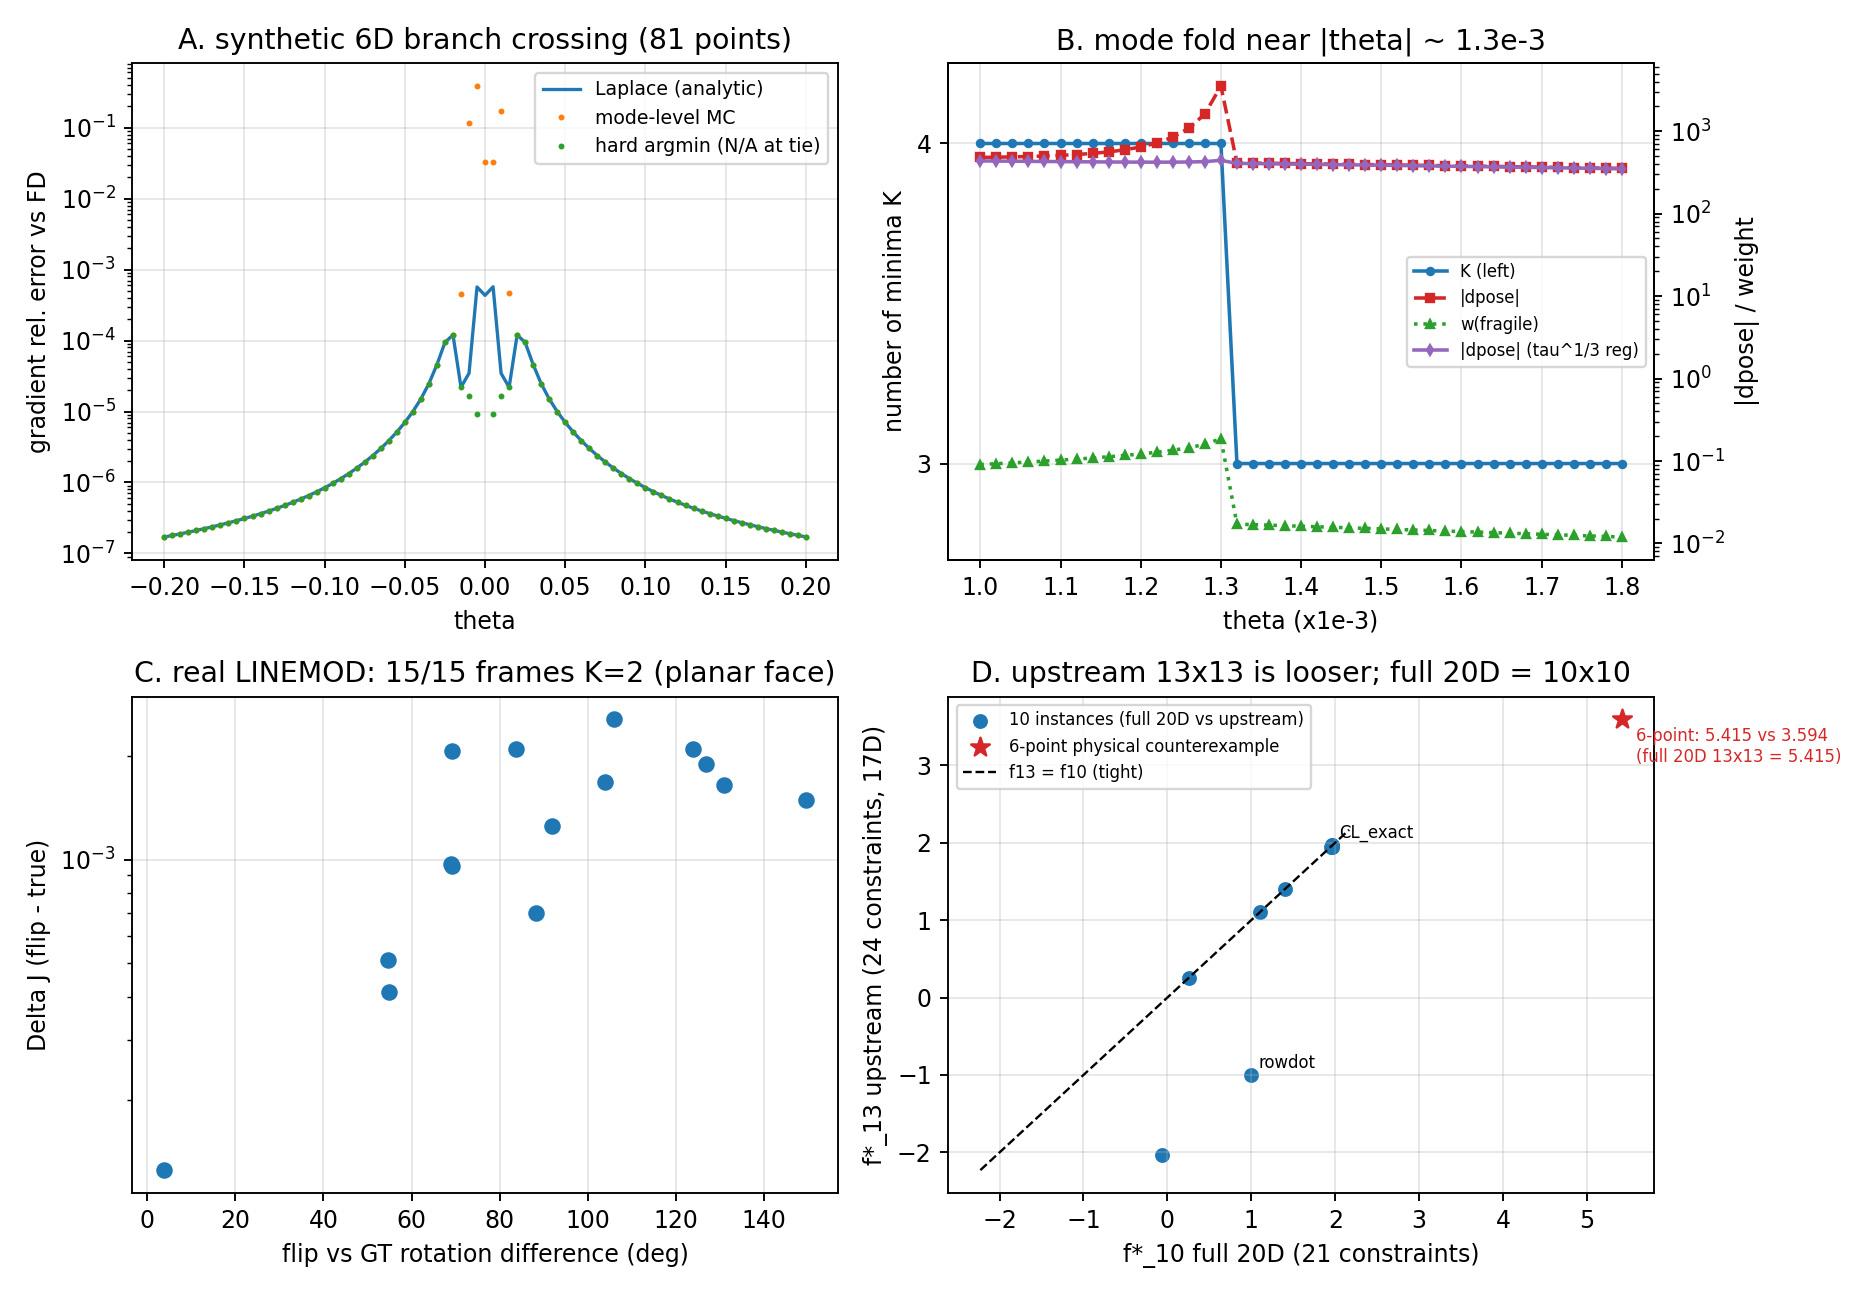
\includegraphics[width=0.92\textwidth]{p1_summary.png}
\caption{四类结果总览。\textbf{(A)} $81$ 点合成 6D 交叉上，解析 Laplace 层、模态级 MC 估计与硬 argmin 的梯度相对误差随 $\theta$ 的变化（交叉处为 N/A）；Laplace 曲线无跳变，硬映射有跳变。\textbf{(B)} $|\theta|\sim1.3\times10^{-3}$ 附近的实测 6D 折叠：极小个数 $K$、位姿映射跳变 $\|d\phi\|$（标准与 $\tau^{1/3}$ 正则化）以及脆弱模态的 Laplace 权重随 $\theta$ 的变化，横轴尺度为 $1.3\times10^{-3}$；模态在 $\theta_f$ 处消失，$\|d\phi\|$ 在该处尖峰。\textbf{(C)} 真实 LINEMOD 帧：目标间隙 $\Delta J$（翻转模态减真模态）与翻转-真值旋转差的关系；$15$ 帧均有 $K=2$。\textbf{(D)} $10$ 个 SDP 实例与 $8$ 个扰动上，上游 24 约束 $13\times13$ 值与完整 20 维 $10\times10$ 值的对比，六点物理反例（星号）将二者分开：$5.415$（完整 20 维）对 $3.594$（上游）。}
\label{fig:p1summary}
\end{figure*}

\begin{table}[t]
\centering
\caption{$81$ 点交叉网格各区间上解析 Laplace 层、模态级 MC 基线与硬 argmin 的梯度相对误差，以及 MC 位姿散布（$\tau=0.01$，FD $h=10^{-4}$，模态级 MC $n=200$、$20$ 个种子，CPU）。每项为区间内网格点的中位数。$\theta=0$ 处的硬 argmin 项为 N/A，因为全局分支在 $\pm h$ 内切换。}
\label{tab:main6d}
\footnotesize
\setlength{\tabcolsep}{4pt}
\begin{tabular}{@{}l r l l l l@{}}
\toprule
区间 & $n$ & Laplace & MC & 硬 argmin & MC 标准差\\
\midrule
远区 & 61 & 4.74e-07 & 4.74e-07 & 4.74e-07 & 2.76e-16\\
近区 & 19 & 3.46e-05 & 9.40e-05 & 2.23e-05 & 2.89e-16\\
交叉点 & 1 & 4.34e-04 & 3.26e-02 & N/A & 1.07e-01\\
\bottomrule
\end{tabular}
\end{table}

网格包含 $61$ 个远区点、$19$ 个近区点与单个交叉点（名义边界 $|\theta|=0.05$ 与 $0.005$）。由此可得三点观察。

\begin{enumerate}
\item \textbf{远离交叉处三种方法一致。} 远区三种方法的相对误差中位数均为 $4.74\times10^{-7}$，MC 位姿散布中位数为 $2.76\times10^{-16}$：全局模态几乎承载全部 Laplace 质量，采样器只看到一个模态。
\item \textbf{Laplace 的优势仅出现在交叉处。} 近区硬 argmin 仍有定义，且中位误差最小（$2.23\times10^{-5}$），优于 Laplace 与 MC；MC 散布中位数为 $2.89\times10^{-16}$，但逐点最大值为 $3.41\times10^{-2}$。$\theta=0$ 处硬 argmin 项为 N/A，Laplace 项受 FD 限制（见下文），MC 误差为 $3.26\times10^{-2}$，位姿散布为 $1.07\times10^{-1}$。
\end{enumerate}

\textbf{$4.34\times10^{-4}$ 是 FD 截断而非方法误差。} 对 Richardson 外推 FD，$\theta=0$ 处为 $1.8\times10^{-7}$，而对 $h=10^{-4}$ 的普通中心 FD 为 $4.3\times10^{-4}$；序列 $4.34\times10^{-8}$（$h=10^{-6}$）、$4.34\times10^{-6}$（$h=10^{-5}$）、$4.34\times10^{-4}$（$h=10^{-4}$）说明了同一点。近区行同样受 FD 限制：$\theta=0.01$ 处 $h=10^{-6}$ 给出 $3.46\times10^{-9}$，而 $h=10^{-4}$ 给出 $3.46\times10^{-5}$。对 $|\theta|\ge0.05$，$h=10^{-5}$ 的误差至多 $7.0\times10^{-8}$。解析梯度在交叉处与 Richardson FD 一致到 $1.8\times10^{-7}$，而不是 $4\times10^{-4}$。

\textbf{硬 argmin 是阶跃映射，Laplace 映射不是。} 随 $\delta\to0$（$\delta=10^{-3},10^{-4},10^{-5}$），$\theta=0$ 两侧的硬位姿跳变保持 $2.86$，而 Laplace 跳变线性衰减（$9.73\times10^{-1}$、$1.00\times10^{-1}$、$1.00\times10^{-2}$），FD 斜率为 $\approx502$，即真实导数。在中心 FD 有定义处，硬映射与 Laplace 一样自洽（非切换情形的中位数为 $1.2\times10^{-4}$），但在恰好交叉的情形中有一半在 $\pm h$ 内切换分支。图~\ref{fig:maintable} 给出逐点误差与 MC 散布。

\begin{figure}[t]
\centering
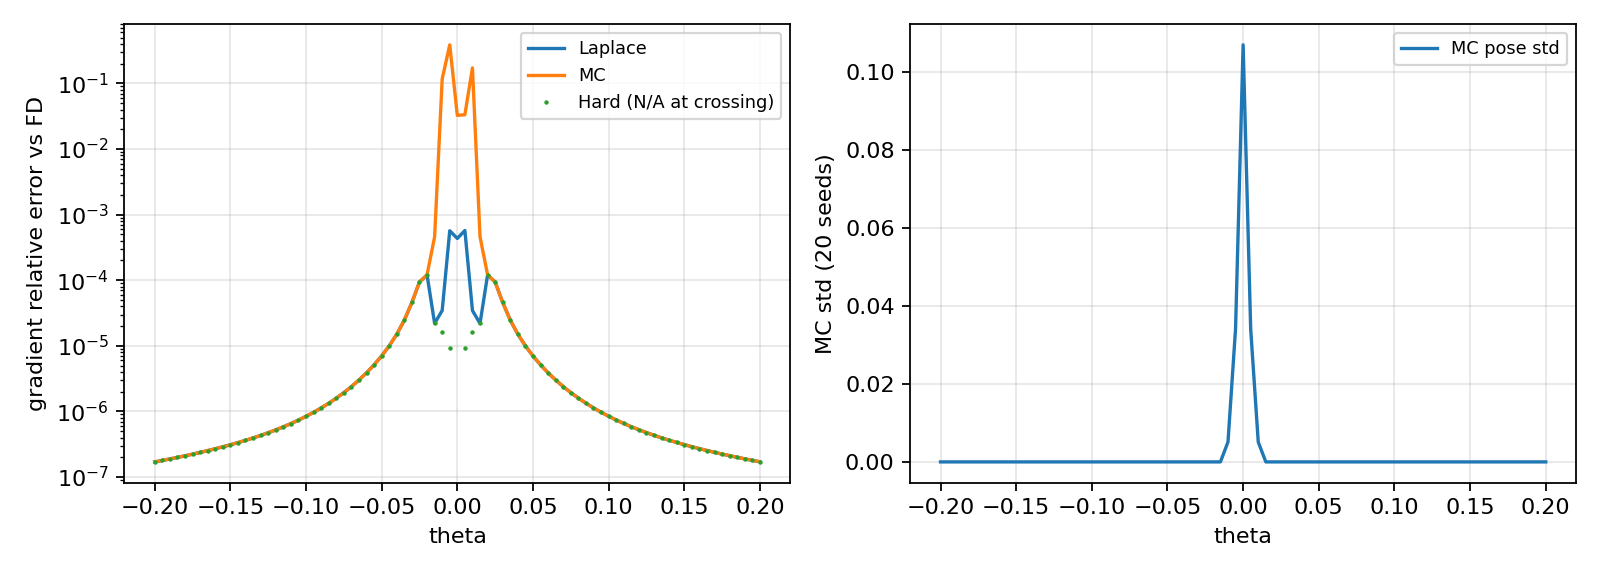
\includegraphics[width=\columnwidth]{main_table.png}
\caption{$81$ 点 6D 交叉网格上的主表诊断。左：解析 Laplace 层（蓝）、模态级 MC 估计（橙）与硬 argmin（绿点；在 FD 参考切换分支的精确交叉处为 N/A）相对沿分支 FD 的梯度误差。右：$20$ 个种子上的 MC 位姿标准差，除 $\theta=0$ 附近窄窗外基本为零。}
\label{fig:maintable}
\end{figure}

\textbf{MC 基线无偏，但在固定预算下噪声较大。} 对同一平滑目标，$n=200\times3$ 个种子给出的逐种子梯度相对误差中位数为 $0.05$（$20$ 种子均值 $7.7\times10^{-3}$），各鲁棒性条件下位姿标准差中位数为 $0.09$，而解析 Laplace 梯度相对 Richardson 参考为 $9.3\times10^{-8}$。这是模态级采样的实测方差代价。

\textbf{模态数与折叠。} 网格上模态数为 $K\in\{1,2,3,4\}$（$K=1$ 有 $30$ 点，$K=2$ 有 $38$ 点，$K=3$ 有 $12$ 点，交叉点为 $K=4$）；这些是上述过滤后的多起点 Newton 返回的局部极小，而非认证根数。光滑性结论限于 $\theta=0$ 与 $|\theta|\lesssim1.3\times10^{-3}$：次极小只在此范围内存在，并在折叠处消失，Laplace 映射在该处不连续（第~\ref{sec:fold6d}~节）。

\subsection{一维精确后验：Laplace 误差为 \texorpdfstring{$O(\tau)$}{O(tau)}}\label{sec:onepd}

\begin{table*}[t]
\centering
\caption{曲率不等的一维标准型中精确后验与双模态 Laplace 的对比（$c=0.25$；$g=0$ 时两个极小位于 $x=\pm1$，曲率为 5 与 3）。$E$ 为 $x$ 的后验均值；误差相对 $[-3,3]$ 上 $2{,}000{,}001$ 点梯形求积。能量为无量纲量，$\Delta J=6.16\times10^{-32}$ 为数值零。}
\label{tab:1d}
\footnotesize
\setlength{\tabcolsep}{5pt}
\begin{tabular}{@{}l l l l l l l l@{}}
\toprule
情形 & $\tau$ & $\Delta J$ & $E_{\mathrm{exact}}$ & $E_{\mathrm{Lap}}$ & $|{\rm err}|$ & $|{\rm err}|/\tau$ & 相对梯度误差\\
\midrule
交叉 & 0.05 & 6.16e-32 & -0.125102 & -0.127017 & 1.92e-03 & 3.83e-02 & 1.77e-02\\
交叉 & 0.02 & 6.16e-32 & -0.126275 & -0.127017 & 7.42e-04 & 3.71e-02 & 6.93e-03\\
交叉 & 0.01 & 6.16e-32 & -0.126649 & -0.127017 & 3.67e-04 & 3.67e-02 & 3.44e-03\\
交叉 & 0.005 & 6.16e-32 & -0.126834 & -0.127017 & 1.83e-04 & 3.66e-02 & 1.71e-03\\
分离 & 0.05 & 4.01e-01 & -1.024203 & -1.031750 & 7.55e-03 & 1.51e-01 & 2.77e-02\\
分离 & 0.02 & 4.01e-01 & -1.029356 & -1.032296 & 2.94e-03 & 1.47e-01 & 1.27e-02\\
分离 & 0.01 & 4.01e-01 & -1.030838 & -1.032296 & 1.46e-03 & 1.46e-01 & 6.27e-03\\
分离 & 0.005 & 4.01e-01 & -1.031570 & -1.032296 & 7.26e-04 & 1.45e-01 & 3.12e-03\\
\bottomrule
\end{tabular}
\end{table*}

期望值误差按 $O(\tau)$ 缩放：交叉处双对数斜率为 1.066，分离盆为 1.036；交叉处 $|{\rm err}|/\tau$ 保持在 $3.66$--$3.83\times10^{-2}$，分离时为 $1.45$--$1.51\times10^{-1}$。梯度误差在表中所列行上随 $\tau$ 单调下降；梯度余项以数值方式检验，而非证明。

\subsection{折叠合并与 \texorpdfstring{$\tau^{1/3}$}{tau^(1/3)} 正则化子}\label{sec:fold1d}

\begin{table*}[t]
\centering
\caption{$\tau=0.01$ 时标准 Laplace 与 $\tau^{1/3}$ 正则化体积因子的对比，$J=x^4/4-ax^2/2$；精确配分由 $[-3.5,3.5]$ 上 $2{,}000{,}001$ 点梯形求积给出。$H=2a$ 为极小处曲率，势垒为 $a^2/4$。}
\label{tab:fold}
\scriptsize
\setlength{\tabcolsep}{2.5pt}
\begin{tabular}{@{}l l l l l l l l@{}}
\toprule
$a$ & $H$ & 势垒 & $Z_{\mathrm{exact}}$ & $Z_{\mathrm{Lap}}$ & Lap 相对误差 & $Z_{\mathrm{reg}}$ & reg 相对误差\\
\midrule
0.50 & 1.00e+00 & 6.25e-02 & 2.6976e+02 & 2.5969e+02 & 3.73e-02 & 2.3556e+02 & 1.27e-01\\
0.20 & 4.00e-01 & 1.00e-02 & 2.3994e+00 & 2.1547e+00 & 1.02e-01 & 1.7371e+00 & 2.76e-01\\
0.10 & 2.00e-01 & 2.50e-03 & 1.2349e+00 & 1.4394e+00 & 1.66e-01 & 9.9871e-01 & 1.91e-01\\
0.05 & 1.00e-01 & 6.25e-04 & 9.7810e-01 & 1.6876e+00 & 7.25e-01 & 9.5017e-01 & 2.86e-02\\
0.02 & 4.00e-02 & 1.00e-04 & 8.6986e-01 & 2.5318e+00 & 1.91e+00 & 1.0019e+00 & 1.52e-01\\
0.01 & 2.00e-02 & 2.50e-05 & 8.3916e-01 & 3.5538e+00 & 3.24e+00 & 1.0358e+00 & 2.34e-01\\
\bottomrule
\end{tabular}
\end{table*}

当 $a\to0$ 时两个极小与鞍点合并，$H\to0$，标准体积因子 $1/\sqrt{H}$ 发散：相对误差从 $a=0.5$ 的 $3.73\times10^{-2}$ 增至 $a=0.02$ 的 $1.91$ 与 $a=0.01$ 的 $3.24$。把 $H$ 换成 $H+\tau^{1/3}$ 后，两个最小 $a$ 处的误差降为 $1.52\times10^{-1}$ 与 $2.34\times10^{-1}$，但并非一致更优：$a=0.5$ 处反而更差（$1.27\times10^{-1}$ 对 $3.73\times10^{-2}$）。正则化形式刻画了合并区域的 $\tau^{1/3}$ 缩放，但并非处处可直接替代。

\subsubsection{实测 6D 折叠}\label{sec:fold6d}

6D 合成映射在交叉附近存在真实折叠。次极小仅在 $|\theta|\lesssim1.3\times10^{-3}$ 时存在（精细折叠扫描给出模态消失点 $\theta_f=1.31\times10^{-3}$，较粗的鲁棒性扫描将其括在 $\approx1.4\times10^{-3}$）；接近折叠时其 $3\times3$ Hessian 行列式降到 $3.35\times10^{-1}$，Laplace 权重从 $0.09$ 升到 $0.187$（该行列式处为 $0.122$），随后模态消失（$K$ 从 4 降到 3）。跨过折叠时位姿映射在一步 $2\times10^{-5}$ 上跳变 $0.31$（在网格加密下保持不变，即真实不连续），$\|d\phi\|$ 峰值达 $3529$，而远离折叠处中位数为 $379$；有效 FD 斜率可达 $1.5\times10^4$。更小的 $\tau$ 或更多起点都不能消除它：$n_{\rm starts}\ge32$ 与 $1024$ 起点的 $K$ 中位数一致（$64$ 个起点在扫描中复现完整模态集），而 $n_{\rm starts}=16$ 在 $10\%$ 的独立抽样中漏掉脆弱模态，一次漏检使位姿最多偏移 $28\%$、梯度最多偏移 $97\%$。因此光滑性与 $O(\tau)$ 精度结论限于 $\theta=0$ 与 $|\theta|\lesssim1.3\times10^{-3}$；多模态 Laplace 映射在极小产生或消失处不连续。

\textbf{折叠的部分修正。} 把 $\det H$ 换成 $\det(H+\epsilon I)$，$\epsilon=\tau^{1/3}$（即上述一维规则，其导数仍为闭式 $\operatorname{tr}((H+\epsilon I)^{-1}\dot H)$），基本消除了\emph{导数}奇异性：$\theta=1.30\times10^{-3}$ 处标准 $\|d\phi\|$ 为 $3529$，正则化后为 $443$；近折叠梯度误差从 $2.90\times10^{-1}$ 降到 $1.19\times10^{-2}$（因子 24）；远离折叠处（$\theta=0.1,0.02$）两种变体在打印精度内一致。它不能消除极小消失导致的\emph{数值}不连续：跨折叠位姿跳变只从 $0.309$ 降到 $0.107$，$K$ 仍从 4 变到 3。因此 Hessian 正则化是折叠邻域的低成本缓解，而跨折叠的连续性结论需要第~\ref{sec:discussion}~节的 Scorer 延拓，或对合并对做局部数值积分。

\subsection{旋转 SDP 证书与三段式 \texorpdfstring{$10\times10$/$13\times13$}{10x10/13x13} 关系}\label{sec:results_sdp}

\begin{table}[t]
\centering
\caption{构造的 $10\times10$ 旋转 SDP 的数值证书（Choi--Lam 四次型加 $2I$；SCS）。间隙为 $f^\star-\mu$，其中 $f^\star=2$ 为四次型在 $\mathbb{S}^3$ 上的解析极小，$\mu$ 为认证对偶值。}
\label{tab:sdp_cert}
\scriptsize
\setlength{\tabcolsep}{3pt}
\begin{tabular}{@{}p{4.6cm} l@{}}
\toprule
量 & 值\\
\midrule
$f^\star$（解析，$C\ge0$，$C(e_0)=0$） & 2.0\\
SDP 原始值 & 1.9658119658\\
对偶 $\mu$ & 1.9658119658\\
对偶证书的 $\lambda_{\min}(Z)$ & $-1.79\times10^{-11}$\\
认证间隙 $f^\star-\mu$ & 0.034188\\
$10^{-6}$ 容差下的 $\operatorname{rank}(X^\star)$ & 6\\
$\lambda_1/\lambda_2$ & 1.451\\
多起点 QPEP 极小（独立校核） & 2.00186\\
具有正间隙的随机扰动 & 8 / 8（0.0453--0.0782）\\
21 条 $SO(3)$ 约束的秩 & 20\\
二次消没理想的维数 & 20\\
\bottomrule
\end{tabular}
\end{table}

$10\times10$ 实例的原始值、对偶值与间隙在打印精度内相互一致；间隙为 $0.034188034\ldots$。这是本文构造（例~\ref{ex:choilam}）。定理~\ref{thm:thirteen} 给出与已发布 $13\times13$ 实现的三段式关系，下述度量分别对应其中每一层。

\begin{table*}[t]
\centering
\caption{上游 24 约束 $13\times13$ 松弛在一般情况下严格松于完整 20 维 $10\times10$ 松弛。$f^\star_{10}$ 为 $10\times10$ 值，$f^\star_{13,\mathrm{up}}$ 为已发布 24 约束实现的值（17 维张成空间）；\texttt{CL\_exact} 为构造的 Choi--Lam 实例，\texttt{rowdot} 为构造的反例。对 \texttt{CL\_exact} 与 \texttt{p6\_data}，真实差值分别为 $3.7\times10^{-11}$ 与 $-2.9\times10^{-10}$，低于六位小数的显示精度。}
\label{tab:13v10}
\footnotesize
\setlength{\tabcolsep}{6pt}
\begin{tabular}{@{}l l l l l l@{}}
\toprule
实例 & $f^\star_{10}$ & $f^\star_{13,\mathrm{up}}$ & $f^\star_{10}-f^\star_{13,\mathrm{up}}$ & 秩 $X_{10}^\star$ & 秩 $X_{13,\mathrm{up}}^\star$\\
\midrule
\texttt{CL\_exact} & 1.965812 & 1.965812 & 3.7e-11 & 6 & 6\\
\texttt{CL\_pert0} & 1.962860 & 1.960078 & 2.8e-03 & 6 & 5\\
\texttt{CL\_pert5} & 1.964571 & 1.950275 & 1.4e-02 & 6 & 4\\
\texttt{rowdot} & 1.000000 & -1.000000 & 2.00 & 10 & 7\\
\texttt{rowdot\_gen} & -0.060192 & -2.029230 & 1.97 & 1 & 4\\
\texttt{p6\_data} & 0.252326 & 0.252326 & 0.0 & 1 & 1\\
\bottomrule
\end{tabular}
\end{table*}

\textbf{解释。} Choi--Lam 等式是对称性的巧合：其上游最优解落在行正交面上，故 $f^\star_{13,\mathrm{up}}=f^\star_{10}=1.9658119658$，两侧秩均为 6，行点积残差至多 $8.8\times10^{-15}$。在八个 $10^{-2}$ 量级的对称破缺扰动后，$8/8$ 个实例满足 $f^\star_{13,\mathrm{up}}<f^\star_{10}$，差值为 $2.5\times10^{-3}$--$1.4\times10^{-2}$，$\operatorname{rank}(X^\star_{13,\mathrm{up}})\in\{4,5\}$ 而 $\operatorname{rank}(X^\star_{10})=6$，上游最优处的 $\max|r_a\cdot r_b|$ 为 $0.59$--$0.88$。构造目标 $Q=-r_1\cdot r_2+\tfrac14I$ 隔离出该机制：它在完整 20 维可行集上是常数 1（$f^\star_{10}=1.000000$），而在上游可达 $-1.000000$（间隙 $2.00$），在 $10^{-2}$ 扰动后仍为 $1.97$。这些度量对应定理~\ref{thm:thirteen} 的第 (2) 层而非第 (1) 层。

\begin{table}[t]
\centering
\caption{区分上游 $13\times13$ 松弛与完整 20 维松弛的六点物理 3D--3D 反例。构造：$p_i=\pm e_1,\pm e_2,\pm e_3$，$y_i=\varepsilon p_i$，$\varepsilon=0.05$；共享矩阵权重 $W$ 满足 $W_{11}=W_{22}=W_{33}=1$、$W_{12}=W_{21}=-0.6$（特征值 $0.4,1.0,1.6>0$），$N=6$，故 $D=0$、$G=6W\succ0$；真值旋转 $R^\star=I_3$ 唯一。中间一列秩由第 (1) 层得到；解析列显式给出秩 1 与 4。}
\label{tab:6point}
\scriptsize
\setlength{\tabcolsep}{3pt}
\begin{tabular}{@{}p{4.1cm} l l@{}}
\toprule
量 & 数值 & 解析\\
\midrule
$f^\star_{10}$（21 条约束，精确秩 20） & 5.41500000 & 5.41500000\\
$f^\star_{13,\mathrm{full}}$（24 + 3 条行正交 = 27 条约束，完整 20 维） & 5.41500000 & 5.41500000\\
$f^\star_{13,\mathrm{up}}$（24 条约束，17 维张成） & 3.59431373 & 3.59430886\\
$f^\star_{10}-f^\star_{13,\mathrm{up}}$ & 1.82068627 & 1.82069114\\
$X^\star_{10}$ / $X^\star_{13,\mathrm{full}}$ / $X^\star_{13,\mathrm{up}}$ 的秩 & 1 / 1 / 4 & 1 / 1 / 4\\
$f_{\rm nonconv}-f^\star_{10}$ & $-8.38\times10^{-13}$ & 0\\
$f_{\rm nonconv}-f^\star_{13,\mathrm{full}}$ & $-3.38\times10^{-13}$ & 0\\
$f_{\rm nonconv}-f^\star_{13,\mathrm{up}}$ & 1.820686 & 1.820691\\
\bottomrule
\end{tabular}
\end{table}

\textbf{该实例为何能区分两者。} 由于 $\pm p_i$ 成对相消，$D=\mathbf{0}$，代价为
\begin{equation}
\begin{split}
J(R,t)={}&2\,\mathrm{tr}(WRR^\top)-4\varepsilon\,\mathrm{tr}(WR)\\
&+2\varepsilon^2\mathrm{tr}(W)+6t^\top Wt .
\end{split}
\label{eq:sixpoint}
\end{equation}
唯一涉及行正交性的项是 $2\,\mathrm{tr}(WRR^\top)=2(\|r_1\|^2+\|r_2\|^2+\|r_3\|^2-1.2\,r_1^\top r_2)$。在完整 20 维约束下，$r_1^\top r_2=0$ 使其成为常数 $6$，而 $-4\varepsilon\,\mathrm{tr}(WR)$ 在 $R=I$ 处取极小，值为 $6(1-\varepsilon)^2=5.415$，故 $f^\star_{10}=f^\star_{13,\mathrm{full}}=f^\star_{\mathrm{QPEP}}=5.41500000$，秩为 1，SCS 水平下间隙为零。上游缺少 $r_1^\top r_2=0$，松弛可取 $\langle r_1^\top r_2\rangle>0$，从而降到 $f^\star_{13,\mathrm{up}}=3.59431373$，秩为 4。

\textbf{解析列中 $4.9\times10^{-6}$ 的差异。} SCS（$\varepsilon=10^{-11}$）给出 $3.59431373$，CLARABEL 给出 $3.59431371$（一致到 $2\times10^{-8}$）；精确有理对偶证书（精确有理 LDU，$\eta=10^{-11}$；最小主元 $1.0\times10^{-11}$，mpmath 60 位 $\lambda_{\min}=+8.0\times10^{-12}$）给出严格下界 $f^\star_{13,\mathrm{up}}\ge3.594313732834$。解析值 $3.59430886$ 比该下界低 $4.87\times10^{-6}$，故不可能是所述 24 约束 SDP 的最优值；$36$ 种自然变体（缩放、子集、布局、归一化、$t$ 块与求解器容差）在 $10^{-8}$ 内都无法复现它，最接近的相差 $4.1\times10^{-6}$。求解器值 $3.5943137\ldots$ 与间隙 $1.8206863\ldots$ 才与该下界一致。定性分离（间隙 $1.82$，秩 $1$ 对 $>1$）不受影响；$\operatorname{rank}(X^\star_{13,\mathrm{up}})$ 在 $10^{-5}$ 阈值下为 $4$，在 $10^{-6}$ 下为 $6$。由于该实例是真实的矩阵加权 3D--3D 代价，Choi--Lam 可实现性问题不适用：间隙是已发布约束集的性质，而三条缺失的行正交约束就是全部原因。

\subsection{导数检验与根计数}\label{sec:rootcount}

\begin{table}[t]
\centering
\caption{反向传播与闭式 $\partial_\theta\log\det H$ 的数值检验。除标注“绝对”外，各项均为相对误差。}
\label{tab:backward}
\scriptsize
\setlength{\tabcolsep}{3pt}
\begin{tabular}{@{}p{3.85cm} p{3.9cm}@{}}
\toprule
检验 & 值\\
\midrule
$E(q)$ 正交性误差 & 1.14e-16\\
$E(q)^\top q$ 误差 & 4.41e-18\\
Euler 恒等式绝对误差 & 5.33e-15\\
黎曼 Hessian，解析对 FD & 9.63e-08\\
隐式 $\partial q^\star/\partial\theta$ 对 FD & 1.51e-07\\
隐式 $\partial t^\star/\partial\theta$ 对 FD & 4.58e-08\\
对映误差（$E$、$H$、$\partial q^\star$、$\partial R$） & 0（精确）\\
Laplace 积分相对误差（$\mathbb{S}^3$ 上的图卡），$\tau=0.2/0.1/0.05/0.025$ & 8.26e-02 / 3.81e-02 / 1.86e-02 / 9.25e-03\\
Laplace 误差对 $\tau$ 的双对数斜率 & 1.05\\
闭式 $\partial_\theta\log\det H$ 对 FD，$5$ 次试验 & 1.65e-09 -- 8.84e-09\\
\quad（最大绝对误差） & 1.59e-09\\
闭式 \texttt{dlogdetH\_dtheta} 对 \texttt{dlogdet\_exact}（修正后） & 8.9e-16\\
闭式 \texttt{dlogdetH\_dtheta} 对沿分支 FD（修正后） & 1.8e-9\\
回归检验：\texttt{dE}/\texttt{dH}/\texttt{dq} & 2.9e-11 / 1.6e-8 / 2.5e-10\\
\bottomrule
\end{tabular}
\end{table}

反向检验在 FD 精度内确认定理~\ref{thm:implicit}；它们并不认证根集。Laplace 常数检验给出斜率 1.05，与定理~\ref{thm:laplace} 的 $O(\tau)$ 结论一致，与精确旋转积分不一致。闭式 $\log\det$ 导数与独立精确导数一致到 $8.9\times10^{-16}$，与沿分支 FD 一致到 $1.8\times10^{-9}$，五次试验中与 FD 一致到 $9\times10^{-9}$ 或更好；回归检验固定 \texttt{dE}/\texttt{dH}/\texttt{dq} 为 $2.9\times10^{-11}$/$1.6\times10^{-8}$/$2.5\times10^{-10}$。

\textbf{根计数与枚举。} 在射影驻点系统上运行全次数同伦，覆盖四个仿射图卡，使用批量复预测-校正与残差校验并集，在 $4/4$ 个实例上找到 \textbf{40 个复射影根}——三个随机对称 $M$ 与 6D 实例 $M(0)$——最大图卡残差 $7.1\times10^{-15}$，每个实例 5.3--8.0 s。每个射影根对应带 $\pm$ 双覆盖的 80 个仿射根。实根情形随实例变化：实射影根为 $26/12/12/20$，实局部极小为 $5/2/2/4$；复根数是通用的（QPEP 作用矩阵界 40），实根数是实例性质。这确认了第~\ref{sec:cert}~节“至多 40 个候选复根”的说法，并认证了代数系统，但不认证 E1/E8 使用的多起点 Newton 枚举器。该枚举器仅在假设 (A2) 下精确：相对 $1024$ 起点参考，$n_{\rm starts}\ge64$ 在扫描中复现模态集，$32$ 与 $K$ 中位数一致，而 $n_{\rm starts}=16$ 在 $10\%$ 的独立抽样中漏掉脆弱模态，故第~\ref{sec:synthetic}~节的模态数是真实计数的下界。\label{sec:enumeration}

\subsection{消融实验}\label{sec:ablations}

\textbf{A. 温度。} 表~\ref{tab:tau} 给出精确 logdet Laplace 层在交叉处、近交叉处与远离交叉处的梯度相对误差。

\begin{table}[t]
\centering
\caption{$\tau$ 扫描（梯度相对误差）。}
\label{tab:tau}
\footnotesize
\setlength{\tabcolsep}{4pt}
\begin{tabular}{@{}l l l l l@{}}
\toprule
$\theta$ & $\tau=0.05$ & 0.02 & 0.01 & 0.005\\
\midrule
+0.000 & 1.20e-03 & 5.84e-04 & 4.34e-04 & 1.51e-03\\
+0.010 & 1.29e-05 & 1.07e-04 & 3.46e-05 & 1.64e-05\\
-0.010 & 1.29e-05 & 1.06e-04 & 3.46e-05 & 1.63e-05\\
+0.100 & 8.47e-07 & 8.46e-07 & 8.46e-07 & 8.46e-07\\
-0.100 & 8.43e-07 & 8.42e-07 & 8.42e-07 & 8.42e-07\\
\bottomrule
\end{tabular}
\end{table}

交叉处 $\tau=0.01$ 时误差最小，$\tau=0.005$ 时回升，这与两个模态近简并时 FD 参考变得不可靠相符；远离交叉处误差约为 $\approx8.5\times10^{-7}$，且与 $\tau$ 无关。

\textbf{B. 体积因子。} 表~\ref{tab:volume} 比较闭式 $\log\det$ 导数、切空间 FD 与从权重中去掉体积因子三种变体。

\begin{table}[t]
\centering
\caption{体积因子变体。\texttt{exact} 为第~\ref{sec:laplace}~节的闭式，\texttt{numeric} 为切空间 FD，\texttt{none} 从权重中去掉 $\tfrac12\log\det H_k$；\emph{位姿差} 与 \emph{梯度差} 为 12 维向量相对 \texttt{exact} 的欧氏范数。}
\label{tab:volume}
\scriptsize
\setlength{\tabcolsep}{3pt}
\begin{tabular}{@{}l l l l l@{}}
\toprule
$\theta$ & 变体 & 梯度相对误差 & 位姿差 & 梯度差\\
\midrule
+0.000 & exact & 4.34e-04 & 0.00e+00 & 0.00e+00\\
+0.000 & numeric & 4.34e-04 & 0.00e+00 & 2.22e-08\\
+0.000 & none & 3.75e-04 & 6.47e-02 & 5.34e+01\\
+0.010 & exact & 3.46e-05 & 0.00e+00 & 0.00e+00\\
+0.010 & numeric & 3.46e-05 & 0.00e+00 & 1.22e-11\\
+0.010 & none & 3.86e-05 & 7.77e-04 & 4.38e-01\\
-0.010 & exact & 3.46e-05 & 0.00e+00 & 0.00e+00\\
-0.010 & numeric & 3.46e-05 & 0.00e+00 & 1.89e-11\\
-0.010 & none & 3.86e-05 & 7.79e-04 & 4.39e-01\\
\bottomrule
\end{tabular}
\end{table}

在交叉处去掉体积因子几乎不改变梯度相对误差，但使平滑位姿改变 $6.47\times10^{-2}$、梯度绝对范数改变 $5.34\times10^{1}$；近交叉处梯度改变 $0.44$。因此该因子对平滑映射并非装饰性的，闭式与切空间 FD 一致到 $2.22\times10^{-8}$ 或更好。

\textbf{C. Top-$K$ 模态截断。} 表~\ref{tab:topk} 只保留权重最高的 $K$ 个模态，并与全部模态之和比较。

\begin{table}[t]
\centering
\caption{Top-$K$ 模态截断（参考：全部模态）。}
\label{tab:topk}
\footnotesize
\setlength{\tabcolsep}{4pt}
\begin{tabular}{@{}l l l l@{}}
\toprule
$\theta$ & $K$ & 位姿差 & 梯度差\\
\midrule
+0.000 & 1 & 1.44e+00 & 4.99e+02\\
+0.000 & 2 & 1.05e-01 & 6.83e+01\\
+0.000 & 3 & 7.95e-02 & 4.93e+01\\
+0.000 & 4 & 0.00e+00 & 0.00e+00\\
+0.010 & 1 & 2.72e-03 & 1.98e+00\\
+0.010 & 2 & 3.02e-05 & 2.65e-02\\
+0.010 & 3 & 0.00e+00 & 0.00e+00\\
+0.010 & 4 & 0.00e+00 & 0.00e+00\\
\bottomrule
\end{tabular}
\end{table}

$\theta=0$ 处只保留最大模态时，位姿相对全模态和改变 $1.44$、梯度改变 $499$；$K=2$ 时降为 $0.105$ 与 $68.3$；$\theta=0.01$ 处 $K=3$ 已在打印精度内精确。因此在打平处必须对所有枚举极小求和，而真实代价包含多少模态仍属实例性质。

\subsection{LINEMOD 真实双模态代价}\label{sec:real}

A 部分在确定性 RANSAC 选出的主平面上构造代价。平面目标具有经典的两重位姿歧义，故方位代价有两个真实极小；变换后落到相机后方的模态（$z\le0$）被剔除。早期一个在单一共享平移下混合两个完整代价的变体没有产生可用行；给每个假设各自的平移（如 B 部分）即可消除折中位姿。

\begin{table*}[t]
\centering
\caption{主平面上的真实双模态方位代价（A 部分）。$15$ 帧均有 $K_{\rm phys}=2$ 个物理极小（$z>0$ 过滤前 $K_{\rm all}=4$）。$w({\rm other})$ 为非硬 argmin 物理模态的 Laplace 权重（$14/15$ 帧为翻转模态；\texttt{000010/72} 为类真值模态）。旋转误差为相对 BOP 真值的度数；Laplace 项为投影弦均值 $\mathrm{Proj}_{SO(3)}(\sum_kw_kR_k)$。}
\label{tab:twomode}
\scriptsize
\setlength{\tabcolsep}{2pt}
\begin{tabular}{@{}l r r l r r r r@{}}
\toprule
帧/图像 & 物体 & $n_{\rm plane}$ & $\Delta J$ & 夹角(°) & $w({\rm other})$ & 硬误差(°) & Lap 误差(°, 投影)\\
\midrule
000010/15 & 10 & 558 & 9.58e-04 & 69.3 & 0.483 & 1.47 & 33.90\\
000010/18 & 10 & 474 & 1.25e-03 & 91.9 & 0.472 & 0.51 & 42.85\\
000010/40 & 10 & 482 & 9.71e-04 & 69.1 & 0.482 & 2.20 & 33.07\\
000010/60 & 10 & 452 & 1.69e-03 & 104.0 & 0.459 & 0.96 & 46.45\\
000010/66 & 10 & 460 & 7.00e-04 & 88.4 & 0.488 & 2.29 & 43.67\\
000010/72 & 10 & 501 & 1.25e-04 & 3.8 & 0.504 & 44.46 & 23.02\\
000010/80 & 10 & 508 & 5.11e-04 & 54.7 & 0.501 & 1.08 & 27.71\\
000010/90 & 10 & 474 & 4.13e-04 & 54.8 & 0.497 & 3.49 & 27.91\\
000011/20 & 11 & 413 & 2.07e-03 & 69.1 & 0.608 & 8.14 & 44.24\\
000011/24 & 11 & 423 & 1.65e-03 & 131.1 & 0.457 & 1.37 & 54.99\\
000011/26 & 11 & 439 & 1.90e-03 & 126.9 & 0.450 & 2.06 & 51.65\\
000011/32 & 11 & 474 & 2.10e-03 & 123.9 & 0.451 & 1.78 & 51.60\\
000011/33 & 11 & 365 & 1.49e-03 & 149.6 & 0.460 & 1.62 & 59.09\\
000011/40 & 11 & 428 & 2.56e-03 & 106.0 & 0.457 & 2.77 & 46.19\\
000011/49 & 11 & 347 & 2.10e-03 & 83.7 & 0.528 & 4.95 & 46.75\\
\bottomrule
\end{tabular}
\end{table*}

\begin{figure}[t]
\centering
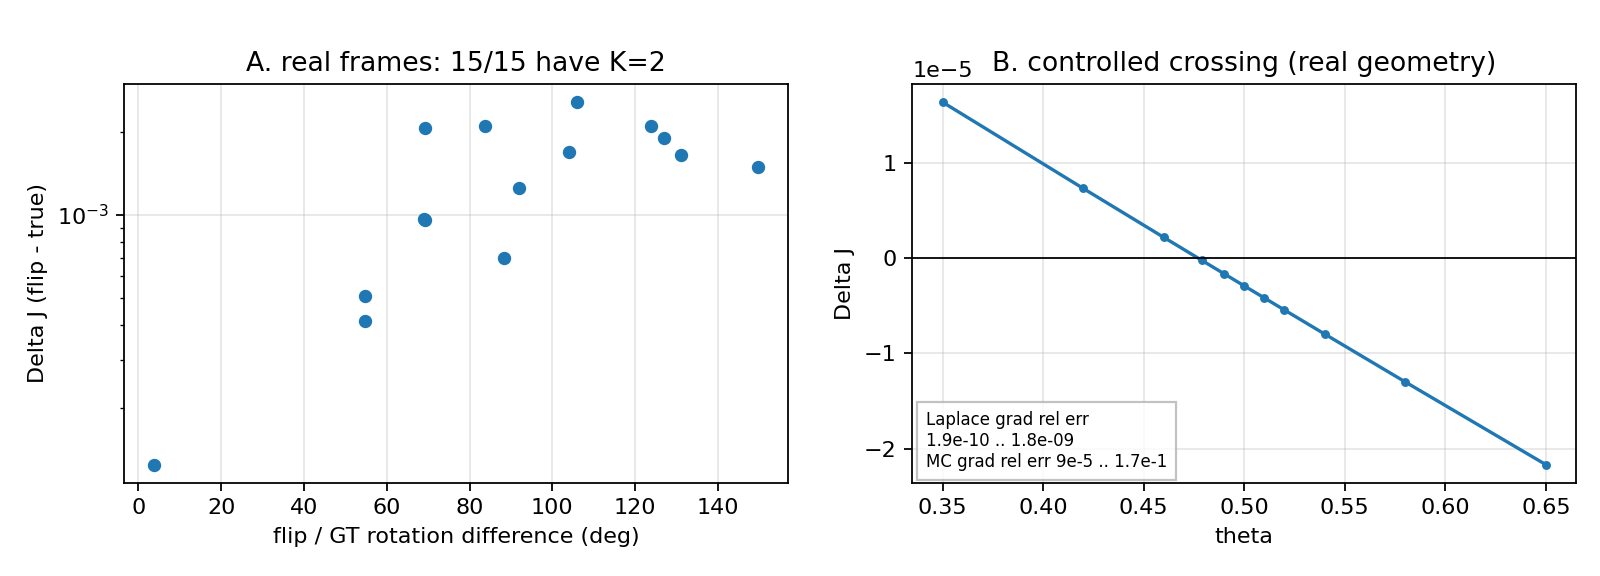
\includegraphics[width=\columnwidth]{two_mode.png}
\caption{真实双模态代价。左：$15$ 帧 LINEMOD 上，翻转模态与类真值模态的目标间隙 $\Delta J$ 对两模态夹角；每帧均有 $K_{\rm phys}=2$，$\Delta J\in[1.25\times10^{-4},2.56\times10^{-3}]$。右：真实几何上的受控横向交叉（B 部分），两个带标签假设按 $J_\theta=(1-\theta)J_{\rm true}+\theta J_{\rm sym}$ 混合；$\Delta J$ 在 $\theta\approx0.475$ 附近变号。插图为解析 Laplace 梯度相对中心 FD 的误差（$1.9\times10^{-10}$--$1.8\times10^{-9}$）与 $400$ 样本 MC 误差（$9\times10^{-5}$--$1.7\times10^{-1}$）。}
\label{fig:twomode}
\end{figure}

由此可得三点。第一，双模态结构可复现：$15/15$ 帧均有 $K_{\rm phys}=2$，$\Delta J\in[1.25\times10^{-4},2.56\times10^{-3}]$，另一模态夹角 $3.8^\circ$--$149.6^\circ$，$w({\rm other})=0.450$--$0.608$。第二，类真值模态在 $14/15$ 帧中是最低 $J$ 的物理模态，故硬 argmin 在这些帧上准确：旋转误差中位数 $2.06^\circ$ $[1.47,3.49]$，ADD-S 中位数 $3.7$ mm $[3.0,4.3]$，只有一帧误差超过 $10^\circ$（\texttt{000010/72}，$44.5^\circ$）。第三，Laplace 后验均值在这些近打平处并非精度提升：投影旋转误差中位数 $44.24^\circ$ $[33.90,46.87]$，相对硬 argmin 的成对偏差 $+36.9^\circ$ $[+27.2,+44.9]$，ADD-S 中位数 $13.9$ mm $[10.3,20.2]$，即约一半质量落在翻转模态。该集合中最小的 Hessian 行列式为 $6.09\times10^{-3}$（\texttt{000011/20}），故翻转模态本身接近折叠。

\begin{table*}[t]
\centering
\caption{$15$ 帧真实数据上的聚合位姿误差与 ADD-S。中位数及帧上 $95\%$ 百分位 bootstrap 置信区间（$1000$ 次重采样）。成对偏差为相对硬 argmin 的逐帧差均值（帧上 $95\%$ 置信区间）；成对旋转偏差中位数为 $+41.8^\circ$。“$\le10^\circ$”统计估计与真值相差不超过 $10^\circ$ 的帧数；对后验均值而言这并不等于“真模态”，因为均值未必是模态。}
\label{tab:aggregate}
\scriptsize
\setlength{\tabcolsep}{3.5pt}
\begin{tabular}{@{}l l l l l l l@{}}
\toprule
方法 & 旋转中位(°) & ADD-S 中位(mm) & ADD 中位(mm) & 旋转偏差(°) & ADD-S 偏差(mm) & $\le10^\circ$ / 真模态\\
\midrule
硬 argmin & 2.06 [1.47, 3.49] & 3.7 [3.0, 4.3] & 5.9 [5.2, 11.1] & --- & --- & 14/15 真模态\\
Laplace（投影） & 44.24 [33.90, 46.87] & 13.9 [10.3, 20.2] & 38.1 [31.0, 41.5] & +36.9 [+27.2, +44.9] & +9.4 [+6.4, +12.6] & 0/15\\
MC（20 种子） & 43.80 [33.90, 47.43] & 14.1 [10.3, 20.0] & 38.0 [31.0, 41.5] & +37.2 [+26.7, +45.0] & +9.4 [+6.4, +12.5] & 0/15\\
\bottomrule
\end{tabular}
\end{table*}

\begin{figure*}[t]
\centering
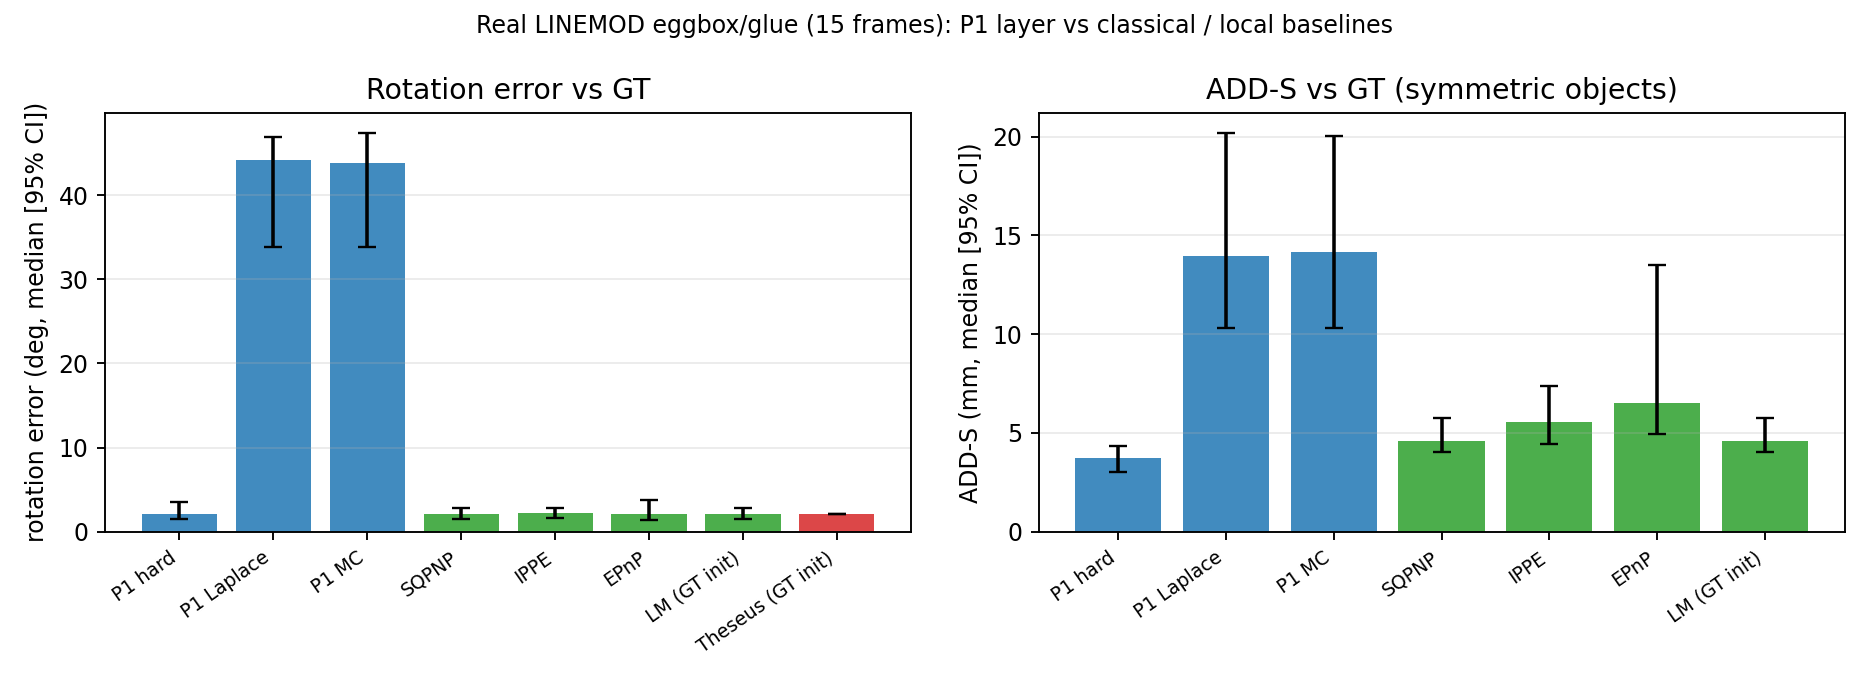
\includegraphics[width=\textwidth]{real_summary.png}
\caption{$15$ 帧真实 LINEMOD \texttt{eggbox}/\texttt{glue} 结果，中位数及 $95\%$ bootstrap 置信区间。左：P1 层（硬 argmin、投影 Laplace 均值、$20$ 种子 MC）与正演/局部参考（SQPNP、IPPE、EPnP、真值初始化的局部 LM、真值初始化的 Theseus）相对 BOP 真值的旋转误差。右：相同方法的 ADD-S（Theseus 未绘出）。硬 argmin 处于经典求解器水平；两个后验均值估计因对两个模态取平均而位于 $44^\circ$ 附近。绿色为前向/局部参考；红色为从真值初始化的局部求解器，不是可部署基线。}
\label{fig:realsummary}
\end{figure*}

$15$ 帧聚合结果见表~\ref{tab:aggregate}。硬 argmin 的均值大于中位数（$5.28^\circ$、$6.0$ mm），原因是个别失败帧；Laplace 的均值为 $42.21^\circ$ 与 $15.5$ mm；平移中位数为 $6.2$ mm（硬）与 $20.2$ mm（Laplace）。MC 估计与 Laplace 相同的平滑均值（$20$ 个种子均值的平均与 Laplace 聚合相差 $0.23^\circ$，在其种子级置信区间内），因此继承该偏差，只额外引入种子噪声（种子间标准差 $1.011^\circ$）。

\begin{table}[t]
\centering
\caption{$15$ 帧真实数据的逐帧 ADD-S（mm；表中“硬/Lap/MC”三列）与 ADD 参考（mm）。“ADD-S 是主要物体空间度量；ADD 为同索引距离，对物体的 $\sim180^\circ$ 对称性不变。}
\label{tab:perframe}
\scriptsize
\setlength{\tabcolsep}{2.5pt}
\begin{tabular}{@{}l r l l l l@{}}
\toprule
帧/图像 & 物体 & 硬 & Lap & MC & ADD（参考）\\
\midrule
000010/15 & 10 & 3.0 & 10.3 & 10.3 & 31.0\\
000010/18 & 10 & 4.3 & 12.2 & 12.3 & 37.6\\
000010/40 & 10 & 6.2 & 9.7 & 9.7 & 31.1\\
000010/60 & 10 & 3.0 & 13.9 & 14.1 & 40.7\\
000010/66 & 10 & 2.7 & 12.1 & 12.0 & 38.0\\
000010/72 & 10 & 12.5 & 8.4 & 8.4 & 22.3\\
000010/80 & 10 & 3.8 & 8.8 & 8.9 & 24.1\\
000010/90 & 10 & 3.1 & 8.5 & 8.4 & 23.3\\
000011/20 & 11 & 13.8 & 22.9 & 22.8 & 72.7\\
000011/24 & 11 & 2.8 & 20.2 & 20.0 & 40.5\\
000011/26 & 11 & 3.7 & 17.6 & 17.5 & 38.1\\
000011/32 & 11 & 3.1 & 19.0 & 19.0 & 41.5\\
000011/33 & 11 & 3.8 & 23.4 & 23.7 & 41.5\\
000011/40 & 11 & 2.2 & 16.8 & 16.7 & 44.7\\
000011/49 & 11 & 22.4 & 28.1 & 28.2 & 75.9\\
\bottomrule
\end{tabular}
\end{table}

逐帧结果有两点值得注意。(i) 在 \texttt{000010/72} 上，硬 argmin 是距真值 $44.5^\circ$ 的模态，而类真值模态距真值 $3.8^\circ$，但 $J$ 高出 $1.25\times10^{-4}$；Laplace/MC 落在两模态之间（$23.0^\circ$、$8.4$ mm），比硬失败更接近真值。这是损失排序在单帧上的偶然，不说明后验均值总体上更准确。(ii) Laplace 位姿的 ADD 是 ADD-S 的 $2$--$3$ 倍（中位数 $38.1$ 对 $13.9$ mm），因为 glue 物体细长，$\sim180^\circ$ 对称性会将其重标；这正是采用 ADD-S 而非 ADD 的原因。

\subsubsection{相同对应点上的经典前向求解器}\label{sec:classical}

表~\ref{tab:classical} 在逐位相同的 $15$ 帧对应点上运行 cv2 的 EPnP、ITERATIVE、SQPNP、IPPE，以及同一方位代价上的普通局部 GN/LM（两个研究已验证逐位一致；真值位姿重投影残差中位数为 $1.47$ px，即约 $1$ px 的最近顶点量化）。这些是前向求解器而非可微层：该 LM 是同一代价上的普通前向优化器，不是 BPnP，也不对其作任何梯度断言。IPPE 在投影到拟合平面的 RANSAC 内点上运行（它要求严格共面，平面性 RMS 为 $0.83$--$1.47$ mm）；其余求解器使用原始内点。

\begin{table*}[t]
\centering
\caption{$15$ 帧真实数据上的经典前向 PnP 基线。中位数及帧上 $95\%$ bootstrap 置信区间（$2000$ 次重采样）。“真模态”统计与真值相差 $10^\circ$ 以内的解。cv2 5.0.0 中 SQPNP 返回单一解（文档针对非 P3P/IPPE 标志，且在全部 $15$ 帧上观测到）；IPPE 返回两个平面解，其中第一个（重投影代价最小）在全部 $15$ 帧上都更接近真值，故 oracle 行与“IPPE 第一个”相同。}
\label{tab:classical}
\scriptsize
\setlength{\tabcolsep}{4pt}
\begin{tabular}{@{}l l l l@{}}
\toprule
方法 & 旋转中位[CI](°) & ADD-S 中位[CI](mm) & 真模态\\
\midrule
EPnP & 2.05 [1.41, 3.71] & 6.5 [5.0, 13.5] & 12/15\\
ITERATIVE（单应初始化 + LM） & 2.07 [1.60, 3.54] & 6.5 [5.7, 8.7] & 11/15\\
SQPNP（单一解） & 2.04 [1.47, 2.77] & 4.6 [4.0, 5.8] & 15/15\\
IPPE（第一个，平面投影） & 2.21 [1.68, 2.76] & 5.5 [4.4, 7.4] & 15/15\\
局部 LM，单位初始化 & 106.01 [69.14, 179.82] & 40.7 [28.0, 1708.7] & 3/15\\
局部 LM，真值初始化 & 2.06 [1.47, 2.77] & 4.6 [4.0, 5.8] & 15/15\\
局部 LM，翻转初始化 & 88.39 [69.08, 106.01] & 23.5 [16.9, 28.0] & 0/15\\
\bottomrule
\end{tabular}
\end{table*}

此处的 ADD-S 列使用 $1000$ 查询/$1000$ 真值顶点估计器，相对表~\ref{tab:aggregate} 的稠密真值 ADD-S 带有 $+1.1$ mm 离散化下限；两列不可直接比较，旋转误差才是可比的精度列。

由此可得三点。(i) 前向点精度处于经典水平：SQPNP/EPnP/ITERATIVE 中位数为 $2.04$--$2.07^\circ$，IPPE 为 $2.21^\circ$，在帧噪声内与硬 argmin 的 $2.06^\circ$ 相当；没有经典求解器接近 Laplace 均值的 $44.2^\circ$。(ii) 单解求解器在某些帧上自信地出错：EPnP 在 $3/15$ 帧、ITERATIVE 在 $4/15$ 帧上偏离真值超过 $10^\circ$（第四帧 \texttt{000011/20} 为 $10.0^\circ$，恰在阈值）；在 \texttt{000010/72} 上两者都返回 $44.3^\circ$/$44.0^\circ$ 的平面翻转解，重投影残差 $0.78$--$0.79$ px，而该翻转解在原始内点上甚至具有更低的方位代价。(iii) 如果没有 $z>0$ 物理性过滤与多起点，局部 LM 从单位初始化失败（$3/15$ 为真，$7/15$ 落到相机后方；中位数 $106^\circ$），从翻转初始化也无法进入真模态（$0/15$）；只有真值初始化能恢复。物理性过滤与枚举在该代价上确实起作用。

\subsubsection{同一代价上的 Theseus LM}\label{sec:theseus}

Theseus 0.2.3（\texttt{LevenbergMarquardt}，float64 CPU）最小化同一方位代价 \cite{pineda2022theseus}；其目标与 numpy 参考一致到 $1.1\times10^{-13}$，解析 Jacobian 与中心差分一致到 $1.3\times10^{-10}$。它是局部优化器：每次调用返回一个位姿，不识别枚举模态集，不返回后验，也不施加 $z>0$ 物理性过滤。

\begin{table*}[t]
\centering
\caption{真实方位代价上的 Theseus LM。“真模态”为与真值相差 $10^\circ$ 以内。随机初始化行在 $15$ 帧上各用 $20$ 个初始化（$300$ 次求解）；多起点行在 $5$ 个代表性帧上各用 $8$ 个初始化（$40$ 次求解），其中位数针对这 $40$ 次试验误差，而非 best-of-8 聚合。}
\label{tab:theseus}
\footnotesize
\setlength{\tabcolsep}{4pt}
\begin{tabular}{@{}l l l p{7.4cm}@{}}
\toprule
协议 & 旋转中位(°) & 真模态 & 结果分解\\
\midrule
真值初始化（15 帧） & 2.06 & 15/15 & 收敛到最近的 P1 模态（\texttt{000010/72} 上为 $3.8^\circ$ 模态，而非全局 argmin）\\
单位初始化（15 帧） & 178.82 & 1/15 & 6 次翻转、8 次其他；8 次在相机后方\\
每帧 20 个随机初始化（300 次求解） & 123.91 & 100/300 (33.3\%) & 57 次翻转、143 次其他、134 次非物理\\
8 初始化 $\times$ 5 帧（40 次求解） & 4.95 & 11/40 (27.5\%) & 无聚合后验；逐试验误差\\
\bottomrule
\end{tabular}
\end{table*}

真值初始化行是局部收敛，而非基线优势。冷启动时 Theseus 返回下降所进入的任一盆地——常是翻转模态或无约束代价的相机后方驻点，正是本文层枚举所剔除的解。它是该近打平代价上自然的无枚举参考，而不是 Laplace 均值的估计器；局部优化在此不能替代模态枚举。

\subsubsection{真实几何上的受控横向交叉}\label{sec:partb}

B 部分消除了早期构造的共享平移问题：两个带标签假设各自消去\emph{自己的}平移，代价按 $J_\theta=(1-\theta)J_{\rm true}+\theta J_{\rm sym}$ 混合。在真实帧 \texttt{000010/15} 上，实测打平点为 $\theta^\star\approx0.475$（构造设计为 $0.5$ 处打平，但重采样使两个带标签代价并非严格对称）；$\Delta J$ 在 $\theta=0.46$ 与 $0.479$ 之间变号，故交叉是横向的，两个极小保持在各自标签位姿的 $\sim2^\circ$ 以内。

\begin{table}[t]
\centering
\caption{真实几何上的受控横向交叉（B 部分，摘录）。\emph{梯度相对误差} 为解析 Laplace 梯度相对层输出中心 FD 的误差；MC 为 $400$ 样本的模态级估计。}
\label{tab:partb}
\scriptsize
\setlength{\tabcolsep}{2.5pt}
\begin{tabular}{@{}l l l l l l@{}}
\toprule
$\theta$ & $\Delta J$ & $w(A)$ & Lap 梯度 & MC 梯度 & $\|d\phi\|$\\
\midrule
0.3500 & +1.64e-05 & 0.50031 & 2.59e-10 & 9.51e-03 & 1.129e-02\\
0.4600 & +2.20e-06 & 0.50004 & 8.61e-10 & 8.94e-05 & 1.123e-02\\
0.4790 & -2.22e-07 & 0.50000 & 7.82e-10 & 1.68e-01 & 1.122e-02\\
0.5000 & -2.89e-06 & 0.49995 & 1.76e-09 & 5.09e-02 & 1.121e-02\\
0.6500 & -2.17e-05 & 0.49960 & 4.03e-10 & 1.10e-02 & 1.112e-02\\
\bottomrule
\end{tabular}
\end{table}

在全部 $11$ 行上，Laplace 梯度与中心 FD 一致到 $1.9\times10^{-10}$--$1.8\times10^{-9}$，而 $400$ 样本模态级 MC 误差为 $8.9\times10^{-5}$--$1.7\times10^{-1}$；硬 argmin 在打平处跳变，其 FD 无定义，故不报告硬梯度。这是闭式反向传播在真实代价上的正确性结果；ADD-S 代理属于 A 部分。

\subsection{运行时间与批处理}\label{sec:compute}

\textbf{仅 CPU。} 所有报告运行均为单进程 CPU 作业。SDP 运行使用 cvxpy 1.9.3/SCS（$\varepsilon=10^{-9}$，\texttt{max\_iters=200000}），对比实验使用 cvxpy 1.7.5/SCS，六点检验使用 $\varepsilon=10^{-11}$、\texttt{max\_iters=10\textasciicircum 6} 的 SCS。真实数据与根计数为短时 CPU 作业：位姿误差/ADD-S 约 $10$ s，经典基线 $3.0$ s，Theseus 对比 $9.5$ s，四个实例的根计数约 $30$ s。

\textbf{计时。} 由 $20$ 次重复，$\theta=0$ 处一次完整合成层调用中位数为 61.9 ms（p95 62.1）：模态枚举占 $88\%$，$K$ 次隐式 $3\times3$ 求解占 $1.6\%$，解析反向（权重梯度与混合）占 $0.1\%$。$\theta=-0.1$ 时整次调用为 17.7 ms。LINEMOD 每帧前向为 24.2--265.9 ms，横向交叉每个 $\theta$（含 FD）为 33.1--42.6 ms。

\textbf{批处理。} 真正的批量多起点 Newton 在批大小 64 时仅比循环快 $1.30\times$（59.9 对 46.2 样本/秒），批大小 8 时为 $0.78\times$，为 1 时为 $0.46\times$：收敛异质性与逐实例分类循环占主导，故需要 GPU 或定制内核才能获得实际吞吐收益。瓶颈是模态枚举，而非 $3\times3$ 求解。

\section{讨论与局限}\label{sec:discussion}

\begin{enumerate}
\item \textbf{SDP 等价的范围与状态。} $10\times10$ Veronese 结果针对的是精确平移消去之后的旋转子问题，它与已发布 $13\times13$ 实现的关系具有已被证明的三部分结构（定理~\ref{thm:thirteen}）。(i) 在完整 20 维理想下，$13\times13$ 松弛\emph{恰好}就是 $10\times10$ 那一个——值相等、秩也相等，由保秩的块 Schur 双射保证——所以一旦理想完备，$10\times10$ 理论确实覆盖了 $13\times13$ 松弛。(ii) 已发布的 24 约束实现只张成 17 维，恰好缺少 $r_1\cdot r_2=r_1\cdot r_3=r_2\cdot r_3=0$，因此一般而言严格更松：$f^\star_{13,\mathrm{up}}\le f^\star_{13,\mathrm{full}}=f^\star_{10,\mathrm{full}}\le f^\star_{\mathrm{QPEP}}$，在对称破缺扰动后有 $8/8$ 个严格间隙（$2.5\times10^{-3}$--$1.4\times10^{-2}$，秩 $\{4,5\}$ 对 6）。(iii) 一个权重为正、真值旋转唯一的 6 点物理 3D--3D 实例以 $1.8207$ 把两者分开，秩为 1 对 4，尽管完整 20D SDP 在该处恰好紧且秩为一。此项已关闭，而不是重新打开：补充材料中“已发布 24 约束松弛与 $10\times10$ 同值”的旧主张才是错误的那个，$10\times10$ 理论不受影响。构造实例的可实现性是另一个问题，仍然开放（第 2 项）。
\item \textbf{Choi--Lam 实例的可实现性。} 构造出的 $M$ 是一个合法的对称代价矩阵，但我们尚未证明它来自真实的 PnP 或矩阵加权对应关系；对\emph{物理}代价矩阵的正测度主张是开放的。在此之前，例~\ref{ex:choilam} 只是关于旋转子问题的陈述，而不是关于 SDPRLayers 生产行为的陈述。第~\ref{sec:results_sdp} 节的 6 点实例\emph{是}物理的，且无需构造目标就分离出了上游实现。
\item \textbf{根枚举。} 前向传播的全局性不会超过求解器本身：漏根、重根与数值消去失败，都会同时破坏“全局”主张与 Laplace 求和。我们把完备性当作假设，并验证残差。计数问题已被测量（$4/4$ 个实例上 40 个复射影根，实根计数 $26/12/12/20$，实局部极小值 $5/2/2/4$）；剩下的是对实际所用枚举器的认证，即多起点牛顿相对同伦在每个实例上的漏根率。逐实例认证的实根计数（带重数的 Sturm/同伦方法）是未来工作。
\item \textbf{Laplace 偏差、折叠与两个折叠定理。} $O(\tau)$ 误差是非一致的。在鞍结（折叠）处模式数发生变化，仅实根的 Laplace 求和甚至不连续。我们对精确平滑后验（第~\ref{sec:laplace} 节）主张光滑性，而对 Laplace 实现只在远离折叠处主张。第~\ref{sec:fold6d} 节测量了两面：在 $\theta=0$ 处 Laplace 映射光滑（其跳变随 FD 斜率 $\approx502$ 线性衰减，而硬映射的跳变保持 $2.86$），但在 $\theta_f\approx1.31\times10^{-3}$ 处存在一个真正的折叠，该处极小值消亡、其权重达到 $0.122$、$\|d\phi\|$ 峰值为 $3529$、位姿映射跳变 $0.31$。更小的 $\tau$ 或更多起点都不能消除该跳变；$\det(H+\tau^{1/3}I)$ 正则化器把导数尖峰降低 24 倍，并把近折叠梯度误差从 $2.9\times10^{-1}$ 降到 $1.2\times10^{-2}$，但只把取值跳变减半（$0.309\to0.107$）。有两个结果解释了原因。

\begin{proposition}[实根代理必然跳变]\label{prop:q5b}
设 $J_\theta$ 在 $\theta_f$ 处经历一个标准的余维 1 折叠（$A_2$）：在它们存在的那一侧（$\theta\to\theta_f^+$），一个次级实极小值 $q_+$ 与邻近的鞍点 $q_-$ 合并为 $q_0$（一个 Hessian 特征值 $\lambda_1(q_+)\to0^+$、横向 Hessian $H_\perp(q_0)\succ0$，并且在别处有一个更深的极小值，满足 $J_0=J_{\theta_f}(q_0)>J_{\rm glob}$），而在另一侧该实极小值消失，于是 $K\to K-1$。那么，任何只对实局部极小值求和、并给合并模式一个正的正则化底权重的代理
\begin{equation}
\tilde w_+^{\rm reg}(\theta_f^+)=\frac{(2\pi\tau)^{3/2}}{\sqrt{\det(H_++\eta(\tau)I_3)}}\,e^{-J_0/\tau},
\label{eq:floorweight}
\end{equation}
在尺度匹配的底 $\eta(\tau)=c_0\tau^{1/3}$ 下，会迫使平滑损失 $\bar\ell_{\rm reg}$ 在 $\theta_f$ 处跳变（其中 $Z_{\rm rest}$ 是其余模式的 Laplace 配分函数）：
\begin{equation}
\begin{split}
&\lim_{\theta\to\theta_f^+}\bar\ell_{\rm reg}-\lim_{\theta\to\theta_f^-}\bar\ell_{\rm reg}\\
&\quad=\frac{\tilde w_+^{\rm reg}(\theta_f^+)}{\tilde w_+^{\rm reg}(\theta_f^+)+Z_{\rm rest}(\theta_f)}\\
&\qquad\times\big(\ell(q_0)-\bar\ell_{\rm rest}(\theta_f)\big)\neq0,
\end{split}
\label{eq:jump}
\end{equation}
并且对 $\eta=c_0\tau^{1/3}$，跳变量为 $\Theta\big(\tau^{1/3}e^{-(J_0-J_{\rm glob})/\tau}\big)$。
\end{proposition}

只有当 $J_0-J_{\rm glob}\gg\tau$ 时它才指数小；当 $J_0-J_{\rm glob}=O(\tau)$ 时它保持 $O(1)$；在任何有限 $\tau$ 下它都非零。这是一个必要性陈述，而不是实现缺陷，也正是 $0.309\to0.107$ 不会趋于零的原因。

\begin{proposition}[复共轭根与 Scorer 延拓]\label{prop:q5c}
40 根作用矩阵求解器把合并对作为复共轭对带过折叠。在正规形
\begin{equation}
J_\theta(u,v)=J_0(\theta)+\tfrac12v^\top H_\perp(\theta)v+\tfrac{c_3(\theta)}{6}u^3-\alpha(\theta)u
\label{eq:normalform}
\end{equation}
中，$c_3>0$、$\alpha(\theta_f)=0$、$\alpha'(\theta_f)>0$（Gromoll--Meyer 分裂）；定义不变量 $J_0=(J(q_+)+J(q_-))/2$ 与 $\zeta(\theta,\tau)=\alpha(\theta)\big(2/c_3(\theta)\big)^{1/3}\tau^{-2/3}$，以及半线 Airy（Scorer）积分
\begin{equation}
\mathcal{S}(\zeta)=\int_0^{+\infty}e^{-s^3/3+\zeta s}\,ds,
\label{eq:scorer}
\end{equation}
它整函数，且 $\mathcal{S}(0)=\Gamma(1/3)/3^{2/3}\approx1.2879$。把两个实根权重换成单个延拓
\begin{equation}
\begin{split}
\tilde w_{\rm fold}(\theta,\tau)={}&\frac{2\pi\tau}{\sqrt{\det H_\perp(\theta)}}\,\tau^{1/3}\Big(\frac{2}{c_3(\theta)}\Big)^{1/3}\\
&\times e^{-J_0(\theta)/\tau}\,\mathcal{S}\big(\zeta(\theta,\tau)\big),
\end{split}
\label{eq:foldweight}
\end{equation}
得到一个在 $\theta_f$ 两侧都是 $C^\infty$ 且取值跳变为零的映射，因为 $(J_0,\alpha,c_3,H_\perp)$ 是特征多项式的对称函数，而 $\mathcal{S}$ 是整函数。对 $\zeta\gg1$，它退化为幸存极小值的普通三维 Laplace 权重 $\tilde w_{\rm fold}=\tilde w_{\rm Lap}(q_+)\big(1+O(\tau/\Delta J_{\rm bar})\big)$；对 $\zeta\ll-1$，它光滑衰减，$\mathcal{S}(\zeta)=|\zeta|^{-1}\big(1+O(|\zeta|^{-3})\big)$。
\end{proposition}

\textbf{该延拓是在不变量层面实现的。} 在 $\theta_f=1.3185\times10^{-3}$ 处的 6D 折叠被双侧跟踪（实极小值/鞍点对与复共轭对），四个不变量 $(J_0,\alpha,c_3,H_\perp)$ 与 $\mathcal{S}(\zeta)$ 在其两侧连续，实测位姿跳变为 $1.21\times10^{-2}$，而标准方法为 $3.04\times10^{-1}$、$\tau^{1/3}$ 方法为 $1.07\times10^{-1}$，即处于光滑映射的导数尺度（$|d\phi|\sim6\times10^2$，跳变/步长为 $6.0\times10^2$ 对 $1.5\times10^4$）。需要注意：把实测不变量等同于正规形只是首阶的（该四次型的四阶系数为 $\approx8.3$），而且这个 6D 折叠很浅（$\Delta J\sim10^{-6}\ll\tau$），因此在折叠\emph{处} Scorer 权重远离其三维 Laplace 极限。主表报告的仍然是仅实根层；它的跳变正是命题~\ref{prop:q5b} 所预言的那个。

\begin{table}[t]
\centering
\caption{6D 折叠处 Scorer 延拓与实根代理的对比（$\theta_f=1.3185\times10^{-3}$、$\tau=0.01$、网格 $\theta_f\pm10^{-4}$、步长 $2\times10^{-5}$）。\emph{跳变}是相邻位姿差的最大值；真正的阶跃在细化下会使\emph{跳变/步长}增长，而光滑映射的\emph{跳变/步长}处于 $|d{\rm pose}|$ 尺度（$\sim6\times10^2$）。}
\label{tab:scorer}
\footnotesize
\setlength{\tabcolsep}{4pt}
\begin{tabular}{@{}l l l l@{}}
\toprule
变体 & 最大跳变 & 跳变 / 步长 & 网格上的 $K$\\
\midrule
标准实根 Laplace & 3.04e-01 & 1.52e+04 & 3--4\\
$\det(H+\tau^{1/3}I)$ 正则化 & 1.07e-01 & 5.34e+03 & 3--4\\
Scorer 延拓 & 1.21e-02 & 6.03e+02 & 4\\
\bottomrule
\end{tabular}
\par\smallskip
\begin{minipage}{\columnwidth}\scriptsize
证据级别：\emph{独立复现（本仓库）}；来源 \path{theory/results/scorer_fold.md}。一维三方校验重现了证明中的 $0.867/0.497/0.3391$，误差 $\le1.6\times10^{-4}$。
\end{minipage}
\end{table}

连续性主张通过网格细化来检验（交错网格，半宽 $10^{-4}$，步长 $d\in\{4\times10^{-5},\ldots,2.5\times10^{-6}\}$）：Scorer 的\emph{跳变/$d$} 在 $d$ 变化 $16\times$ 的范围内保持 $404.3,404.2,404.0,403.7,403.3$（在 $d=2.5\times10^{-6}$ 处没有数值下限），而标准映射的\emph{跳变/$d$} 从 $7.6\times10^{3}$ 增长到 $2.1\times10^{5}$，正则化映射的则从 $2.7\times10^{3}$ 增长到 $4.4\times10^{4}$（一个常数阶跃）。这取代了早先“未做细化检验”的保留意见。因此，折叠邻域落在仅实根 Laplace 层的适用范围之外：要主张连续性，就需要 Scorer 延拓，或对合并对做局部数值积分。

\begin{figure*}[t]
\centering
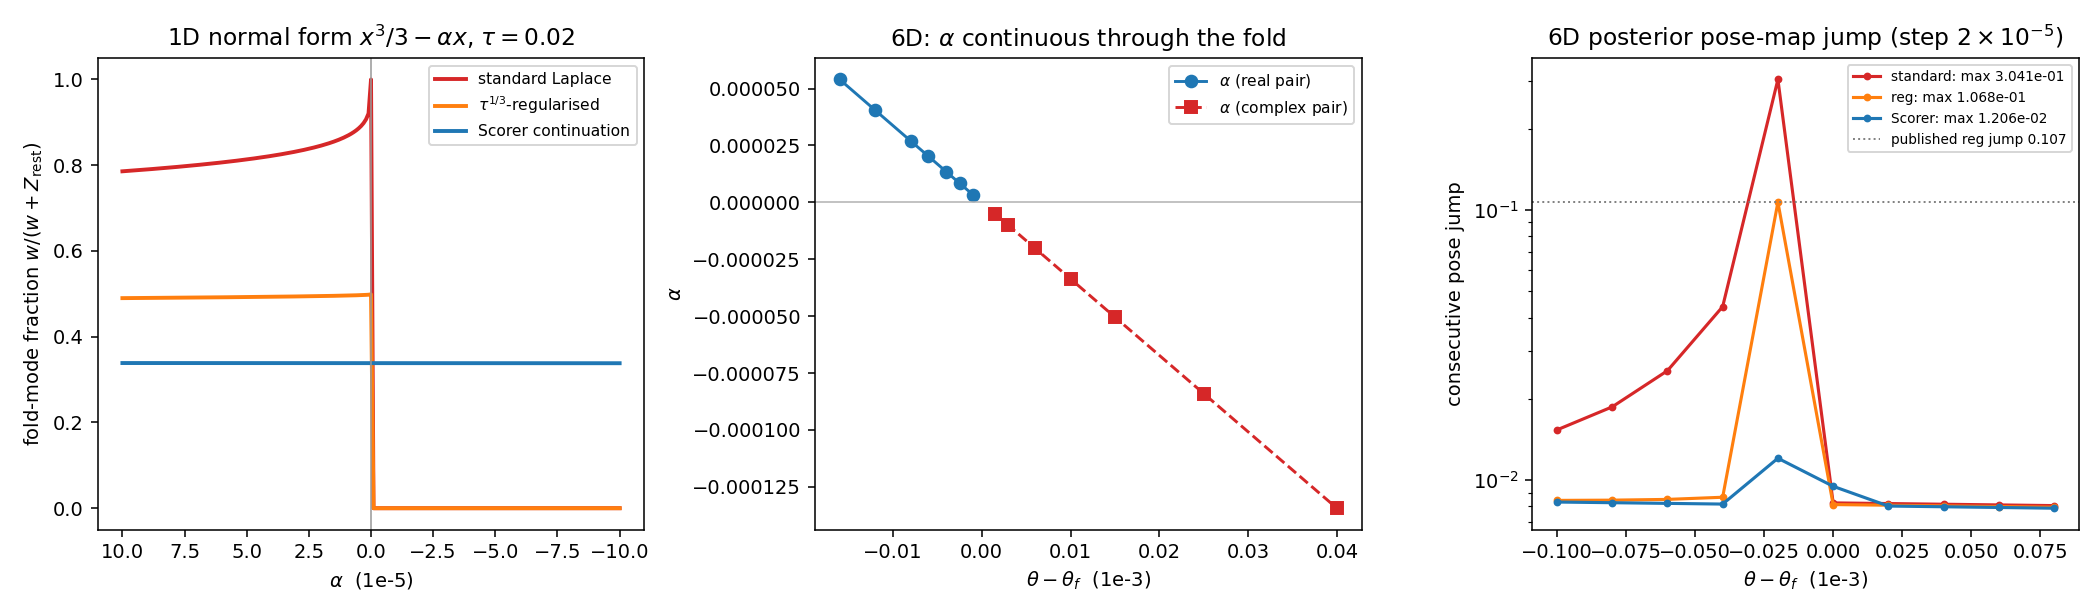
\includegraphics[width=\textwidth]{scorer_fold.png}
\caption{折叠处的 Scorer 延拓。\textbf{左：}一维正规形 $x^3/3-\alpha x$，$\tau=0.02$；折叠模式的权重占比对标准 Laplace 求和而言是不连续的，对 $\tau^{1/3}$ 正则化体积因子从 $0.4959$ 跳到 $0$，而对 Scorer 延拓则是连续的（$0.33838\to0.33834$）。\textbf{中：}$\theta_f=1.3185\times10^{-3}$ 处的 6D 折叠；不变量 $\alpha$ 被穿过折叠跟踪，在实根对/复根对切换处连续。\textbf{右：}最大相邻后验位姿跳变相对 $\theta-\theta_f$：标准映射尖峰到 $3.04\times10^{-1}$，正则化映射到 $1.07\times10^{-1}$，而 Scorer 延拓的峰值为 $1.21\times10^{-2}$，处于光滑映射的导数尺度。}
\label{fig:scorer}
\end{figure*}

\item \textbf{对称物体：一个正结果及其精度代价。} 新的真实数据构造在 15/15 个 LINEMOD \texttt{eggbox}/\texttt{glue} 帧上产生两个真正的模式，而实测结果并不是精度胜利：硬 argmin 在近平局处是准确的（中位数 $2.06^\circ$、ADD-S $3.7$ mm，处于经典前向求解器的水平），而 Laplace 均值被拉向翻转（中位数 $44.24^\circ$、ADD-S $13.9$ mm；配对偏差 $+36.9^\circ$）。这就是该层所做的精度/光滑性取舍，而且对称物体上的行为现在是被测量过的，而不是未被测试的。
\item \textbf{三阶导数。} $\nabla_\theta\log\det H_k$ 需要 $J$ 的三阶 $q$ 导数以及 $q^{(k)}$ 的隐式导数；对四次型而言可以处理，但要正确实现并不简单。它是“$3\times3$ 反向传播”这一口号与完整 Laplace KL 之间的主要差距。
\item \textbf{温度。} $\tau$ 是一个依赖代价尺度的超参数。没有尺度归一化时它不可辨识；有了尺度归一化，$\tau$ 就可以学习。$\tau\to0$ 极限只对后验均值/argmin 恢复确定性梯度，对原始 KL 损失则不然。
\item \textbf{没有不等式约束，也没有外点鲁棒性。} 这些被委托给伴随工作线：该层假设 $G\succ0$ 与固定的加权 Gram 矩阵，不处理非穿透、手性不等式或严重外点。
\item \textbf{GPU 批处理。} 代数根枚举是工程瓶颈；一个批量的 $40\times40$ 复特征值求解器看起来可行，但尚未基准测试。
\end{enumerate}

\section{结论}\label{sec:conclusion}

本文提出 \textsc{Laplace-QPEPLayer}，一个将 QPEP 的四元数代数、$3\times3$ 黎曼隐式微分与多模态 Laplace 后验相结合的可微位姿层。理论核心包括：旋转提升与 Veronese 嵌入之间的精确正交桥梁；21 条标准 $SO(3)$ 约束张成二次 Veronese 理想的证明；$0.034188$ 认证间隙、$\operatorname{rank}(X^\star)=6$ 的 Choi--Lam 实例；联系 $10\times10$ 松弛与已发布 $13\times13$ 松弛的三段式定理；以及具有对映不变性的闭式反向传播。概率核心是精确平移积分与全部枚举旋转极小上的解析 Laplace 和，并给出显式误差阶与失效模式。该设计在推理时无 SDP 提升、无 Monte Carlo 采样、无不等式约束、无抗外点核。

在合成 6D 交叉上，Laplace 映射光滑而硬 argmin 是阶跃映射，Laplace 梯度与 Richardson FD 一致到 $1.8\times10^{-7}$；一维精确后验检验给出 $O(\tau)$ 误差，双对数斜率为 1.066 与 1.036；旋转 SDP 以 $0.034188$ 的间隙得到认证；已发布 24 约束松弛在物理六点实例上松 $1.8207$（$5.415$ 对 $3.59431373$）；全次数同伦在 $4/4$ 个实例上确认 40 个复射影根。

在 $15$ 帧具有真实双模态代价的 LINEMOD 数据上，硬 argmin 在近打平处准确，达到经典 EPnP/SQPNP 水平（中位数 $2.06^\circ$、$3.7$ mm ADD-S），而 Laplace 均值被拉向翻转模态（$44.24^\circ$、$13.9$ mm，偏差 $+36.9^\circ$）。该层换来的是在分支交叉处光滑、确定性且无需采样的梯度，其代价恰是在两个模态近打平的帧上损失位姿精度。


\appendix
\section{21 条二次约束的完备性：维数计数}\label{app:dimcount}

令 $\nu_2:\mathbb{RP}^3\to\mathbb{RP}^9$ 为二次 Veronese 嵌入 $[q]\mapsto[v_2(q)]$，其中 $v_2(q)\in\mathbb{R}^{10}$ 按第~\ref{sec:lift}~节的归一化收集 $q=(q_0,q_1,q_2,q_3)$ 的十个二次单项式；并令
\begin{equation}
\begin{split}
&\mathcal{I}_2\big(\nu_2(\mathbb{RP}^3)\big)\\
&\quad=\Big\{M\in\operatorname{Sym}^2(\mathbb{R}^{10}):\\
&\qquad v_2(q)^\top Mv_2(q)\equiv0\quad\forall q\in\mathbb{R}^4\Big\}.
\end{split}
\label{eq:app-ideal}
\end{equation}
考虑线性求值映射
\begin{equation}
\begin{split}
&\Phi:\operatorname{Sym}^2(\mathbb{R}^{10})\longrightarrow\mathbb{R}[q_0,q_1,q_2,q_3]_4,\\
&\Phi(M)(q):=v_2(q)^\top Mv_2(q).
\end{split}
\label{eq:app-phi}
\end{equation}

\textbf{(i) 核。} 由 \eqref{eq:app-ideal}，$\ker\Phi=\mathcal{I}_2(\nu_2(\mathbb{RP}^3))$。

\textbf{(ii) 满射性。} 目标空间由满足 $a_0+a_1+a_2+a_3=4$ 的四次单项式 $q_0^{a_0}q_1^{a_1}q_2^{a_2}q_3^{a_3}$ 张成。每个这样的单项式可分解为两个二次单项式之积 $m_1(q)m_2(q)$：取整数 $0\le b_i\le a_i$ 且 $\sum_ib_i=2$（因 $\sum_ia_i=4$ 故可行），令 $m_1=\prod_iq_i^{b_i}$、$m_2=\prod_iq_i^{a_i-b_i}$。每个 $m_\ell$ 至多差一个常数就是 $v_2$ 的某个坐标；故存在指标 $r,s$ 与常数 $c_r,c_s$ 使
\begin{equation}
\begin{split}
m_1(q)m_2(q)&=c_rc_s\,(v_2)_r(q)(v_2)_s(q)\\
&=\Phi\!\left(\tfrac{c_rc_s}{2}(e_re_s^\top+e_se_r^\top)\right)(q).
\end{split}
\label{eq:app-monomial}
\end{equation}
于是像包含全部基单项式，$\Phi$ 为满射。

\textbf{(iii) 计数。} 源空间与目标空间的维数分别为
\begin{equation}
\begin{split}
\dim\operatorname{Sym}^2(\mathbb{R}^{10})&=\frac{10\cdot11}{2}=55,\\
\dim\mathbb{R}[q_0,q_1,q_2,q_3]_4&=\binom{4+4-1}{4}=\binom74=35 .
\end{split}
\label{eq:app-dims}
\end{equation}
由秩-零化度定理与满射性，
\begin{equation}
\dim\mathcal{I}_2\big(\nu_2(\mathbb{RP}^3)\big)=\dim\ker\Phi=55-35=20 .
\label{eq:app-20}
\end{equation}
这是关于映射 $\Phi$ 的陈述；它对于 21 条 $SO(3)$ 约束矩阵的完备性是必要而不充分的，因为尚未说明这些矩阵达到该计数。

\textbf{(iv) 21 条约束达到 20 维。} 设 $A_i\in\mathbb{S}^{10}$（$i=1,\dots,21$）为定理~\ref{thm:ideal} 的约束在 $x_R$ 坐标下的矩阵，$N_i:=(2U)^\top A_i(2U)$ 为其在 $v_2$ 坐标下的拉回。由于 $x_R=2Uv_2$ 且 $x_R(q)^\top A_ix_R(q)\equiv0$ 在 $\mathbb{S}^3$ 上成立，
\begin{equation}
v_2(q)^\top N_iv_2(q)=x_R(q)^\top A_ix_R(q)\equiv0\quad\forall q\in\mathbb{R}^4,
\label{eq:app-pullback}
\end{equation}
故 $N_i\in\ker\Phi$。对 $N_1,\dots,N_{21}$ 的 55 个系数向量作精确有理高斯消元，得
\begin{equation}
\operatorname{rank}\{N_1,\dots,N_{21}\}=20 .
\label{eq:app-rank}
\end{equation}
唯一的线性相关是迹恒等式
\begin{equation}
\begin{split}
&\sum_{a=1}^{3}\big(\|c_a\|^2-x_0^2\big)-\sum_{a=1}^{3}\big(\|r_a\|^2-x_0^2\big)\\
&\quad=\operatorname{tr}(R^\top R)-\operatorname{tr}(RR^\top)\equiv0 .
\end{split}
\label{eq:app-dependency}
\end{equation}
因此 $\operatorname{span}\{N_i\}$ 是 20 维核 \eqref{eq:app-20} 的 20 维子空间，故等于该核，21 条约束张成完整的二次消没理想。该计数对约束集敏感：仅六个非对角内积的秩为 $15$，这正是已发布 24 约束实现的约束亏缺并非记账细节的原因。

\section{Haar 测度、双覆盖与 Laplace 常数}\label{app:haar}

\subsection*{局部 Jacobian \texorpdfstring{$dR=8\,du$}{dR=8du}}

设 $q^{(k)}\in\mathbb{S}^3$，$E_k\in\mathbb{R}^{4\times3}$ 满足 $E_k^\top q^{(k)}=0$、$E_k^\top E_k=I_3$。取正规坐标
\begin{equation}
q(u)=\frac{q^{(k)}+E_ku}{\sqrt{1+\|u\|_2^2}},\qquad u\in\mathbb{R}^3 .
\label{eq:app-chart}
\end{equation}
在 $u=0$ 处 $\dot q(0)=E_k\dot u$，且体坐标系纯虚四元数为 $(q^{(k)})^{-1}\dot q(0)=[0,\dot u^\top]^\top$。在双覆盖 $\pi:\mathbb{S}^3\to SO(3)$（$R(q)v=qvq^{-1}$）下求导得
\begin{equation}
\mathrm{d}\pi_{q^{(k)}}\big(E_k\dot u\big)=R(q^{(k)})\,[2\dot u]_\times ,
\label{eq:app-dpi}
\end{equation}
故体角速度为 $\omega=2\dot u$。对一般标准正交切基 $E_k=E_R(q^{(k)})Q_k$（$Q_k\in O(3)$），有 $\partial\omega/\partial u|_{u=0}=2Q_k$。取与轴角向量欧氏测度对应的双不变体积元 $\mathrm{d}R=\mathrm{d}\omega_1\wedge\mathrm{d}\omega_2\wedge\mathrm{d}\omega_3$，则
\begin{equation}
\mathrm{d}R=\left|\det\frac{\partial\omega}{\partial u}\right|_{u=0}\mathrm{d}u
=|\det(2Q_k)|\,\mathrm{d}u=8\,\mathrm{d}u,
\label{eq:app-jac}
\end{equation}
且 $\operatorname{Vol}(SO(3))=8\pi^2$。
全局归一化一致：$\int_{SO(3)}f\,\mathrm{d}R=\frac12\int_{\mathbb{S}^3}f(R(q))\,8\,\mathrm{d}\sigma(q)=4\int_{\mathbb{S}^3}f\,\mathrm{d}\sigma$，取 $f=1$ 得 $\frac12\cdot8\cdot2\pi^2=8\pi^2$。

\subsection*{双覆盖与逐模态因子}

在非退化模态 $q^{(k)}$ 附近，正规坐标 \eqref{eq:app-chart} 中单个叶片上的 Laplace 积分为 $\int e^{-J/\tau}\mathrm{d}u=(2\pi\tau)^{3/2}(\det H_k)^{-1/2}e^{-J_k/\tau}(1+O(\tau))$。乘 Jacobian \eqref{eq:app-jac} 得每叶片 $8(2\pi\tau)^{3/2}(\det H_k)^{-1/2}e^{-J_k/\tau}$。对映两片 $\pm q^{(k)}$ 是 $\mathbb{S}^3$ 上 $J$ 与 $H$ 相同的两个不同点，双覆盖给出因子 $1/2$；两个因子精确抵消，故每个 $SO(3)$ 模态贡献
\begin{equation}
8(2\pi\tau)^{3/2}\frac{e^{-J_k/\tau}}{\sqrt{\det H_k}} .
\label{eq:app-permode}
\end{equation}
于是，在未归一化测度 $\mathrm{d}R$ 下，
\begin{equation}
\begin{split}
&\int_{SO(3)}e^{-J_{\mathrm{red}}/\tau}\mathrm{d}R\\
&\quad=8(2\pi\tau)^{3/2}\sum_{k=1}^K\frac{e^{-J_k/\tau}}{\sqrt{\det H_k}}\big(1+O(\tau)\big),
\end{split}
\label{eq:app-rotint}
\end{equation}
即 \eqref{eq:rotationint}。若取概率 Haar 测度 $\mathrm{d}\mu_{\mathrm{Haar}}=\mathrm{d}R/(8\pi^2)$，则同一积分再除以 $8\pi^2$。

\subsection*{\texorpdfstring{$Z_{\mathrm{Lap}}$}{Z\_Lap} 的绝对常数}

将 \eqref{eq:app-rotint} 与精确平移积分 \eqref{eq:gaussint} 结合，并取概率 Haar 测度，
\begin{equation}
\begin{split}
Z_{\mathrm{Lap}}(\theta)&=\frac{(\pi\tau)^{3/2}}{\sqrt{\det G}}\cdot\frac{(2\pi\tau)^{3/2}}{\pi^2}\sum_{k=1}^K\frac{e^{-J_k/\tau}}{\sqrt{\det H_k}}\\
&=\frac{2\sqrt2\,\pi\tau^3}{\sqrt{\det G}}\sum_{k=1}^K\frac{e^{-J_k/\tau}}{\sqrt{\det H_k}} .
\end{split}
\label{eq:app-zlap}
\end{equation}
若取未归一化测度 $\mathrm{d}R$，右端还要乘与 $\theta$ 无关的因子 $8\pi^2$。该因子在固定 $\tau$ 时为常数，在 $w_k$ 与 $\nabla_\theta L_{\tau\text{-KL}}$ 中相消；只有 \eqref{eq:app-zlap} 应作为绝对常数引用。

\subsection*{包络定理与 \texorpdfstring{$\log\det H_k$}{log det H\_k} 的完整导数}

设 $J_{\mathrm{red}}(q;\theta)=v_2(q)^\top M(\theta)v_2(q)$，$q^{(k)}(\theta)$ 为非退化驻点，$E_k^\top\nabla_qJ_{\mathrm{red}}=0$，$H_k=E_k^\top(\nabla^2J_{\mathrm{red}}-4J_kI_4)E_k\succ0$。由于 $\mathrm{d}q^{(k)}\in\operatorname{range}(E_k)$ 且 $\operatorname{range}(E_k)=(q^{(k)})^\perp$，
\begin{equation}
\nabla_\theta J_k=v_2(q^{(k)})^\top\big(\partial_\theta M\big)v_2(q^{(k)}) .
\label{eq:app-envelope}
\end{equation}
记 $\xi_k=-H_k^{-1}E_k^\top\partial_\theta\nabla_qJ_{\mathrm{red}}$，使 $\partial_\theta q^{(k)}=E_k\xi_k$，由链式法则得
\begin{equation}
\begin{split}
&\partial_\theta\log\det H_k\\
&\quad=\operatorname{tr}\!\Big[H_k^{-1}E_k^\top\Big(\partial_\theta\nabla^2J_{\mathrm{red}}\\
&\qquad+\mathrm{D}_q\big(\nabla^2J_{\mathrm{red}}\big)[E_k\xi_k]
-4\,\partial_\theta J_k\,I_4\Big)E_k\Big].
\end{split}
\label{eq:app-dlogdet}
\end{equation}
有两个精确简化。反对称标架旋转项在 $\operatorname{tr}(H_k^{-1}\dot H_k)$ 中由迹的循环性相消，因为 $\log\det H_k$ 在切基的正交变换下不变。法向弯曲项由 Euler 齐次性消失：$\nabla^2J_{\mathrm{red}}q^{(k)}=3\nabla_qJ_{\mathrm{red}}(q^{(k)})$，故 $E_k^\top\nabla^2J_{\mathrm{red}}q^{(k)}=3E_k^\top\nabla_qJ_{\mathrm{red}}=0$。最后，$J_{\mathrm{red}}$ 是四次型，故 $\mathrm{D}_q(\nabla^2J_{\mathrm{red}})[\delta q]$ 关于 $q$ 线性，\eqref{eq:app-dlogdet} 中的缩并每个模态仅需 $O(1)$。这就是简写 \eqref{eq:dlogdet} 与梯度 \eqref{eq:annealedgrad} 背后的完整导数。


\bibliographystyle{plain}
\bibliography{refs}

\end{document}
